% Options for packages loaded elsewhere
\PassOptionsToPackage{unicode}{hyperref}
\PassOptionsToPackage{hyphens}{url}
%
\documentclass[
  english,
  man,floatsintext]{apa6}
\usepackage{amsmath,amssymb}
\usepackage{lmodern}
\usepackage{ifxetex,ifluatex}
\ifnum 0\ifxetex 1\fi\ifluatex 1\fi=0 % if pdftex
  \usepackage[T1]{fontenc}
  \usepackage[utf8]{inputenc}
  \usepackage{textcomp} % provide euro and other symbols
\else % if luatex or xetex
  \usepackage{unicode-math}
  \defaultfontfeatures{Scale=MatchLowercase}
  \defaultfontfeatures[\rmfamily]{Ligatures=TeX,Scale=1}
\fi
% Use upquote if available, for straight quotes in verbatim environments
\IfFileExists{upquote.sty}{\usepackage{upquote}}{}
\IfFileExists{microtype.sty}{% use microtype if available
  \usepackage[]{microtype}
  \UseMicrotypeSet[protrusion]{basicmath} % disable protrusion for tt fonts
}{}
\makeatletter
\@ifundefined{KOMAClassName}{% if non-KOMA class
  \IfFileExists{parskip.sty}{%
    \usepackage{parskip}
  }{% else
    \setlength{\parindent}{0pt}
    \setlength{\parskip}{6pt plus 2pt minus 1pt}}
}{% if KOMA class
  \KOMAoptions{parskip=half}}
\makeatother
\usepackage{xcolor}
\IfFileExists{xurl.sty}{\usepackage{xurl}}{} % add URL line breaks if available
\IfFileExists{bookmark.sty}{\usepackage{bookmark}}{\usepackage{hyperref}}
\hypersetup{
  pdftitle={Cognitive Music Listening Space: A Multivariate Approach},
  pdfauthor={Brendon Mizener1, Mathilde Vandenberghe2, Herve Abdi1, \& Sylvie Chollet2},
  pdflang={en-EN},
  pdfkeywords={keywords},
  hidelinks,
  pdfcreator={LaTeX via pandoc}}
\urlstyle{same} % disable monospaced font for URLs
\usepackage{graphicx}
\makeatletter
\def\maxwidth{\ifdim\Gin@nat@width>\linewidth\linewidth\else\Gin@nat@width\fi}
\def\maxheight{\ifdim\Gin@nat@height>\textheight\textheight\else\Gin@nat@height\fi}
\makeatother
% Scale images if necessary, so that they will not overflow the page
% margins by default, and it is still possible to overwrite the defaults
% using explicit options in \includegraphics[width, height, ...]{}
\setkeys{Gin}{width=\maxwidth,height=\maxheight,keepaspectratio}
% Set default figure placement to htbp
\makeatletter
\def\fps@figure{htbp}
\makeatother
\setlength{\emergencystretch}{3em} % prevent overfull lines
\providecommand{\tightlist}{%
  \setlength{\itemsep}{0pt}\setlength{\parskip}{0pt}}
\setcounter{secnumdepth}{-\maxdimen} % remove section numbering
% Make \paragraph and \subparagraph free-standing
\ifx\paragraph\undefined\else
  \let\oldparagraph\paragraph
  \renewcommand{\paragraph}[1]{\oldparagraph{#1}\mbox{}}
\fi
\ifx\subparagraph\undefined\else
  \let\oldsubparagraph\subparagraph
  \renewcommand{\subparagraph}[1]{\oldsubparagraph{#1}\mbox{}}
\fi
% Manuscript styling
\usepackage{upgreek}
\captionsetup{font=singlespacing,justification=justified}

% Table formatting
\usepackage{longtable}
\usepackage{lscape}
% \usepackage[counterclockwise]{rotating}   % Landscape page setup for large tables
\usepackage{multirow}		% Table styling
\usepackage{tabularx}		% Control Column width
\usepackage[flushleft]{threeparttable}	% Allows for three part tables with a specified notes section
\usepackage{threeparttablex}            % Lets threeparttable work with longtable

% Create new environments so endfloat can handle them
% \newenvironment{ltable}
%   {\begin{landscape}\begin{center}\begin{threeparttable}}
%   {\end{threeparttable}\end{center}\end{landscape}}
\newenvironment{lltable}{\begin{landscape}\begin{center}\begin{ThreePartTable}}{\end{ThreePartTable}\end{center}\end{landscape}}

% Enables adjusting longtable caption width to table width
% Solution found at http://golatex.de/longtable-mit-caption-so-breit-wie-die-tabelle-t15767.html
\makeatletter
\newcommand\LastLTentrywidth{1em}
\newlength\longtablewidth
\setlength{\longtablewidth}{1in}
\newcommand{\getlongtablewidth}{\begingroup \ifcsname LT@\roman{LT@tables}\endcsname \global\longtablewidth=0pt \renewcommand{\LT@entry}[2]{\global\advance\longtablewidth by ##2\relax\gdef\LastLTentrywidth{##2}}\@nameuse{LT@\roman{LT@tables}} \fi \endgroup}

% \setlength{\parindent}{0.5in}
% \setlength{\parskip}{0pt plus 0pt minus 0pt}

% \usepackage{etoolbox}
\makeatletter
\patchcmd{\HyOrg@maketitle}
  {\section{\normalfont\normalsize\abstractname}}
  {\section*{\normalfont\normalsize\abstractname}}
  {}{\typeout{Failed to patch abstract.}}
\patchcmd{\HyOrg@maketitle}
  {\section{\protect\normalfont{\@title}}}
  {\section*{\protect\normalfont{\@title}}}
  {}{\typeout{Failed to patch title.}}
\makeatother
\shorttitle{Music Descriptor Space}
\keywords{keywords\newline\indent Word count: X}
\usepackage{lineno}

\linenumbers
\usepackage{csquotes}
\usepackage{caption}
\ifxetex
  % Load polyglossia as late as possible: uses bidi with RTL langages (e.g. Hebrew, Arabic)
  \usepackage{polyglossia}
  \setmainlanguage[]{english}
\else
  \usepackage[main=english]{babel}
% get rid of language-specific shorthands (see #6817):
\let\LanguageShortHands\languageshorthands
\def\languageshorthands#1{}
\fi
\ifluatex
  \usepackage{selnolig}  % disable illegal ligatures
\fi
\newlength{\cslhangindent}
\setlength{\cslhangindent}{1.5em}
\newlength{\csllabelwidth}
\setlength{\csllabelwidth}{3em}
\newenvironment{CSLReferences}[2] % #1 hanging-ident, #2 entry spacing
 {% don't indent paragraphs
  \setlength{\parindent}{0pt}
  % turn on hanging indent if param 1 is 1
  \ifodd #1 \everypar{\setlength{\hangindent}{\cslhangindent}}\ignorespaces\fi
  % set entry spacing
  \ifnum #2 > 0
  \setlength{\parskip}{#2\baselineskip}
  \fi
 }%
 {}
\usepackage{calc}
\newcommand{\CSLBlock}[1]{#1\hfill\break}
\newcommand{\CSLLeftMargin}[1]{\parbox[t]{\csllabelwidth}{#1}}
\newcommand{\CSLRightInline}[1]{\parbox[t]{\linewidth - \csllabelwidth}{#1}\break}
\newcommand{\CSLIndent}[1]{\hspace{\cslhangindent}#1}

\title{Cognitive Music Listening Space: A Multivariate Approach}
\author{Brendon Mizener\textsuperscript{1}, Mathilde Vandenberghe\textsuperscript{2}, Herve Abdi\textsuperscript{1}, \& Sylvie Chollet\textsuperscript{2}}
\date{}


\authornote{

Add complete departmental affiliations for each author here. Each new line herein must be indented, like this line.

Enter author note here.

The authors made the following contributions. Brendon Mizener: Stimuli creation, Survey design \& creation, Data collection \& processing, Statistical analyses, Writing - Original draft preparation; Mathilde Vandenberghe: Original concept, Survey design \& creation; Herve Abdi: Writing - Review \& Editing, Statistical guidance; Sylvie Chollet: Original concept.

Correspondence concerning this article should be addressed to Brendon Mizener, 800 W. Campbell Rd., Richardson Tex. E-mail: \href{mailto:bmizener@utdallas.edu}{\nolinkurl{bmizener@utdallas.edu}}

}

\affiliation{\vspace{0.5cm}\textsuperscript{1} University of Texas at Dallas\\\textsuperscript{2} YNCREA}

\abstract{
Participants with either French or American nationality responded to surveys featuring novel music stimuli and evaluated those musical excerpts using either adjectives or quantitative musical dimensions. We opted during the design phase of this study to permit lesser control of various parameters in order to reach a greater sample. We did not control how participants listened to the stimuli, but they were encouraged to use headphones or listen in a quiet listening environment. Participants were also able to complete the survey using a mobile device. Results were analyzed using correspondence analysis (CA), Hierarchical cluster analysis (HCA), Multiple Factor Analysis (MFA), and Partial Least Squares Correlation (PLSC). All except the HCA used Bootstrapping and Permutation testing for inferences. Significant differences were revealed in how French and American lay listeners responded to the excerpts.
}



\begin{document}
\maketitle

\#top
Music listening is a complex cognitive activity that involves many judgments per second. Listeners continuously evaluate incoming information and compare it with that which came before. These judgments involve many different dimensions of music related to both the technical and affective aspects of this acoustic medium. While these two aspects of music are theoretically distinct, in practice there is a great deal of interplay between the two. Listeners respond affectively to technical aspects of music, and composers use those technical things to reflect their internal emotional states. Assessing the interplay between the two is quite a task, because it's difficult to isolate specifically which musical mechanisms affect listeners in specific ways, to say nothing of the individual associations that participants bring to the table.
Research into the emotion of music, specifically, is a well-trod topic. See, for example, (\textbf{Juslin2010?}). With advances in computational power and complexity, this research domain has given rise to studies in the realms of computational neuroscience and electrical engineering, as researchers attempt to classify which physical characteristics of music correspond to which emotions in music. This `Music Emotional Retrieval' (MER) is an interesting computational exercise, it ignores the semantics and associations of music that resonate with listeners. In the behavioral domain, researchers focus on asking participants to rate music with sliders, specifically asking the participants to evaluate `arousal' and `valence,' features that were found very early to be defining elements of the first two dimensions of music affective perception {[}Osgood; Wedin{]}. This is useful, but limiting, as it provides fine-grained detail on the level of arousal or valence a given stimulus provides, but does not qualify that information. Similarly, studies that ask participants to cluster stimuli depend on greater levels of interpolation from the researchers in determining affective impact.
A review of the literature surrounding music perception quickly reveals a limited perspective. Firstly, the participants in these experiments are largely WEIRD (Western, Educated, Industrialized, Rich, and Democratic). The participant pool becomes even smaller when you realize that researchers commonly use students in their departments as participants, either psychology or music, or in some cases marketing or business. This practice inherently biases the sample towards wealth and the ethnic majority, as representation and access to higher education remains an issue. In terms of stimuli, although there is a database of over 20000 previously used musical excerpts (\textbf{Warrenburg2020?}), the vast majority of those are either western or popular music. These stimuli are also often presented under strict laboratory control, which we respectfully submit does not reflect an ecologically valid process for listening.
Multidimensional scaling (MDS) was introduced fairly early in this field as a means of evaluating the perceptual space around musical excerpts (\textbf{Wedin1969?}; \textbf{Wedin1972?}). Studies in this vein have continued to date, including examples like (\textbf{Droit-Volet2013?}) or (\textbf{Roda2014?}), which continue to provide evidence supporting the existence of the valence-arousal plane. (\textbf{Roda2014?}) specifically investigates what the dimensions beyond valence and arousal may be. However, these studies and their analyses have been limited in their attempts at analyzing and visualizing the factor space of their stimuli. These and others plot the stimuli in a factor space, using the valence-arousal plane as \emph{a priori} defined axes. The use of the \emph{a priori} defined axes is not per se a negative aspect of this, but the fact that these analyses are unable to evaluate both the music and semantic dimensions simultaneously. It's difficult therefore to evaluate the semantic and holistic music cognitive/emotional sensory space.
Earlier studies in this domain evaluated how various technical aspects of music correspond to emotions for the purpose of induction, (see (\textbf{BrunerII1990?}) for a summary) but the musical characteristics listed and they way they were investigated don't fully capture the dimensionality that composers consider when writing music. Also, many of the studies that investigate from this perspective impose strict limitations on how the stimuli vary, which is useful for illuminating very specific effects of a single musical element or characteristic, but makes it impossible to evaluate interactions between any musical variables. Assessing the interplay between the technical aspects of music and descriptive/affective requires a fine - grained approach that is able to evaluate the correlations and covariates between many dimensions simultaneously.
The gradual increase in complexity of studies in behavior and cognition, coupled with the rise of questions about the universality of experience and the democratization of science, compels us to find novel ways of investigating the experience of music. We as researchers need to develop experimental paradigms that are robust to violations in experimental procedure, in order to access a larger part of the population, The burden to define testing parameters and provide clear analysis becomes much greater. Controlling for extraneous variables becomes a problem in and of itself. The balance between establishing a broad research question and analyzing with precision is very delicate. Additionally, accessing a broader population is necessary, but the concerns of parametrization and control are similar.

\hypertarget{present-questions-methods-of-analysis}{%
\subsection{Present questions \& methods of analysis}\label{present-questions-methods-of-analysis}}

In this study, we attempt to address three specific issues with the field as a whole: mode of investigation, sample \& size, and analysis. The initial motivation for this study came from a cross-modal study investigating cross modal sensory mapping between gustation perception, specifically beer, and music perception. Prior iterations of this experiment suggest that a wide variety in musical stimuli was necessary to determine any correlations or differences. As such, this study is designed to investigate whether a music cognitive listening space can be established using this paradigm, to allow cross-modal comparison. Details on participant sample and sample size are included below.
Additionally, we present methods of analysis drawn from other domains that we have found to be useful in illuminating various new aspects of these questions that may help guide future hypothesis testing.
Additional questions arise from the study itself: are there significant differences in how participants from different nationalities (and by extension musical cultures) perceive, or, more precisely, describe music? Are there parallels in how music is evaluated using music non-specific descriptors and music-specific qualities? Because this study was designed to be exploratory in nature, we feel it would be poor scientific practice to present specific hypotheses.\\
\#\# Analysis
For the main analyses of the first two experiments we used Correspondence Analysis, which is similar to Principal Components Analysis (PCA), except that it allows for the analysis of qualitative data. This analysis technique was selected because it allows for biplots; the simultaneous display of row and column factor scores in the same factor space. The biplot specifically allows plotting the excerpts in the same space as the descriptors, which provides a clear, quick, visual reference for what excerpts or musical pieces fall in to what quadrant or area of the cognitive space. The third experiment required a different analytical technique. Because we were comparing two data tables, we used a Partial Least Squares Correlation (PLSC), a technique commonly used in imaging studies to compare brain fMRI and behavioral data. Other analyses included MDS, to plot the participants' individual factor scores in their own factor space, as well hierarchical cluster analyses on both excerpts and adjectives to see what clusters arose during ratings. We also performed a post-hoc multiple factor analysis using the results of the second survey after seeing that there were significant differences between french and american participants. This is included in the discussion section of the second experiment.

After cleaning and preprocessing, the data for each participant will take the form of a pseudo contingency table. These individual tables are all compiled into a `brick,' or three-dimensional array of data with Observations (stimuli) on the rows, variables (musical qualities or adjectives) on the columns, and participants on the third dimension, which we will refer to as `pages' here. This brick is then summed across pages into a single table, so that any given cell contains the total number of times a participant selected a given adjective or quality to match with a stimulus.
From this point there are two sets of data that can be analyzed. The first is the 3D array, which can be analyzed using various distance analyses, to evaluate differences between the participants using grouping variables extracted from the demographics surveys. The other is the pseudo contingency table, which can be analyzed using various multivariate techniques.
- what processing steps are needed

\hypertarget{methods}{%
\section{Methods}\label{methods}}

\hypertarget{participants}{%
\subsection{Participants}\label{participants}}

Participants (N = 604) were recruited similarly for both Experiments 1 and 2, and thus are discussed simultaneously here. Participants for this study were recruited in multiple ways, all of which represent convenience sampling. The participants in the United States (n = 292) were recruited using the traditional method of offering experimental participation credit, and also via social media. French participants (n = 312) were recruited by word of mouth, email, and social media. The only restrictions on participation were that the participant must have self-reported normal hearing. We recognize that although we suggest that data collected in this way have a much greater hypothetical reach, the data here represent a) a convenience sample, b) that is limited to participants that have access to the internet. Both of these specific limitations could be remedied when designing and implementing future research.\\
The population we recruited was different for the two experiments. For Experiment 1, we specifically sought out highly trained musicians (n = 84) with ten years or more of music training. We recruited this population for two reasons: firstly, as a validation step, to ascertain whether the stimuli truly reflected the composer's intent. Secondly, we had the goal of evaluating how the musical qualities of the stimuli, as evaluated by the trained participants, correlated with the adjectives selected by those who participated in the adjectives survey. Participants were recruited for Experiment 2 (n = 520) without regard to level of music training.\\
Of the responses to Experiment 1, 51 were removed to incomplete data (nf = 45, nA = 6), leaving a total of 33 for the analysis. Of the responses to experiment 2, 160 were removed for not completing the survey (nF = 140, nA = 20), leaving a total of 360. Of the responses to the survey administered in the US, participants were excluded from analysis if they indicated a nationality other than American. ``Asian-American,'' for example, was included, but ``Ghanian'' was not. This left a total of 312 participants for analysis across both experiments.
All recruitment measures were approved by the UT Dallas IRB.

\hypertarget{material}{%
\subsection{Material}\label{material}}

\hypertarget{stimuli}{%
\subsubsection{Stimuli}\label{stimuli}}

All stimuli were original musical excerpts composed for this study. They were designed to evaluate a number of musical dimensions and control for others (e.g., timbre). The stimuli were all string quartets, in order to control for the confounding factor that different instruments are fundamentally described in different ways. All stimuli were between 27s and 40s long, with an average length of 32.4s. The intent was to have all stimuli be around 30s long while preserving musical integrity. All stimuli were composed between April 13 and June 18, 2020.

\hypertarget{surveys}{%
\subsubsection{Surveys}\label{surveys}}

There were two separate surveys presented to participants. The survey used in Experiment 1 (hereafter: Qualities Survey/QS) evaluated the musical stimuli on concrete musical qualities like meter and genre. The survey used in Experiment 2 (hereafter: Adjectives Survey/AS) asked participants to evaluate the stimuli using adjectives using the CATA paradigm. Both surveys also captured participants' demographic data, including age, gender, nationality, occupation, and musical experience.\\
The qualities assessed in the QS were selected from standard music-theoretical descriptors of music. For example, when rating the excerpts on tempo, participants were asked to rate the excerpt using the scale \emph{Very Slow}, \emph{Slow}, \emph{Moderately Slow}, \emph{Moderate}, \emph{Moderately Fast}, \emph{Fast}, and \emph{Very Fast}. The full list of musical qualities and associated levels is in {[}supplementary materials?{]}. The words for the AS were selected using (\textbf{Wallmark2019?}) as a guide and in consult with a French professional musician. Some words were initially selected in French and some in English. In all cases, words were selected for which there was a clear French (vis-a-vis English) translation. The words and their translations are listed in {[}supplementary materials?{]}.

\hypertarget{procedure}{%
\subsection{Procedure}\label{procedure}}

Participants were provided with a link to either the AS or the QS. Both surveys were administered using Qualtrics. After standard informed consent, participants listened to 15 excerpts and answered questions. Demographic survey questions followed the experimental task. Participants were instructed to listen to the excerpts presented either using headphones or in a quiet listening environment, but that was not strictly controlled, nor was it part of the survey. Participants in Experiment 1 answered 10 questions per excerpt, rating the excerpts using the qualities and scales provided. Participants in Experiment 2 answered a single question per excerpt, in which they selected any and all adjectives that they felt described the excerpt.

\hypertarget{cata-paradigm}{%
\subsection{CATA paradigm}\label{cata-paradigm}}

While not invented by (\textbf{Katz1933?}), the Check-All-That-Apply (CATA) investigative paradigm was used in that study to evaluate racial stereotypes among college students. As an method it's not terribly common in the psychological sciences any more, but it has been and continues to be used widely to ``obtain rapid product profiles'' (\textbf{Meyner2014?}) from participants. It is also commonly used in sensory evaluation. In this method, participants are asked to select any and all adjectives from a list that describe a given stimulus. This allows researchers to collect a lot of data about a given stimulus without placing demand on the participants.

\hypertarget{data-processing-and-analysis}{%
\subsection{Data processing and analysis}\label{data-processing-and-analysis}}

Raw data were cleaned and processed in Excel and R. This included translating all French responses to English for ease of analysis. Data were cleaned and transformed into a pseudo contingency table for each participant. Whereas a contingency table would be when a participant selects only one option from a list for each stimulus, resulting in a table with one and only one one (1) per row, a pseudo contingency table has as many ones as items selected for a given stimulus. Because we are using the CATA technique, a one (1) at the intersection of each row or column indicates that the participant selected that adjective or musical quality for that stimulus. A zero means that they did not. These individual tables were all compiled into into two `bricks,' or three-dimensional arrays of data with Observations (stimuli) on the rows, variables (musical qualities or adjectives) on the columns, and participants on the third dimension, which we will refer to as `pages' here. Each array was then summed across pages into a single summary pseudo-contingency table, so that any given cell contained the total number of times a participant selected a given adjective or quality for a given stimulus.
The arrays with participants on the third dimension were analyzed using distance analyses to evaluate differences between the participants using grouping variables extracted from the demographics surveys. The summed tables were analyzed using Correspondence Analysis. Since we did not use \emph{a priori} grouping variables for the excerpts, the summed tables were evaluated using hierarchical cluster analyses to see what groupings arose during evaluation.
A final analysis (Partial Least Squares Correlation, see (\textbf{Abdi2013a?})) evaluated correlations between the two summed data tables to see what information was shared between the two tables.
For each of these analyses, variance is extracted in the form of eigenvalues. The individual factor scores are plotted relative to these eigenvalues, which form the axes of the maps shown below. The dimensions extracted in this process are by definition orthogonal and share no information. For the sake of efficiency, for each of the analyses below, we focus on the first two dimensions.

\hypertarget{correspondence-analysis}{%
\subsubsection{Correspondence Analysis}\label{correspondence-analysis}}

Correspondence Analysis (CA) is similar to Principal Components Analysis (PCA), except that it allows for the analysis of qualitative data. Because of the organization of the data, this technique allows for a biplot of both rows and columns in a single factor space. In addition to factor plots, we used permutation tests and bootstrapping for statistical inferences. Multiple correspondence analysis

\hypertarget{partial-least-squares-correlation}{%
\subsubsection{Partial Least Squares Correlation}\label{partial-least-squares-correlation}}

Partial Least Squares Correlation (PLSC) analyzes two data tables either on the same observations (rows) or variables (columns). This technique is commonly used in neuroimaging studies to evaluate correlations between matrices of imaging data and of behavioral or task data (\textbf{Krishnan2011?}). In this case, we are evaluating the correlation and covariance between the the stimuli, which are the observations (rows) for both data tables.

\hypertarget{results}{%
\section{Results}\label{results}}

\hypertarget{experiment-1-musical-qualities-survey}{%
\subsection{Experiment 1: Musical Qualities Survey}\label{experiment-1-musical-qualities-survey}}

\begin{verbatim}
## [1] "It is estimated that your iterations will take 1 minutes."
## [1] "R is not in interactive() mode. Resample-based tests will be conducted. Please take note of the progress bar."
## ================================================================================
\end{verbatim}

\hypertarget{participants-1}{%
\subsubsection{Participants}\label{participants-1}}

The scree plot below shows the eigenvalues for the distance analysis between musical experts. The usual guideline of analyzing only dimensions with eigenvalues greater than one seems prohibitive here, as all dimensions except the last have \(\lambda\) \textgreater{} 1. For the purposes of this experiment, we've opted to focus on the first two dimensions, with \(\lambda\) = 9.06 and \(\lambda\) = 7.52, respectively. This suggests that each of the participants is contributing similarly to the dimensionality of this analysis. This analysis revealed no significant difference between the experts based on any of the grouping variables used.

\begin{figure}

{\centering 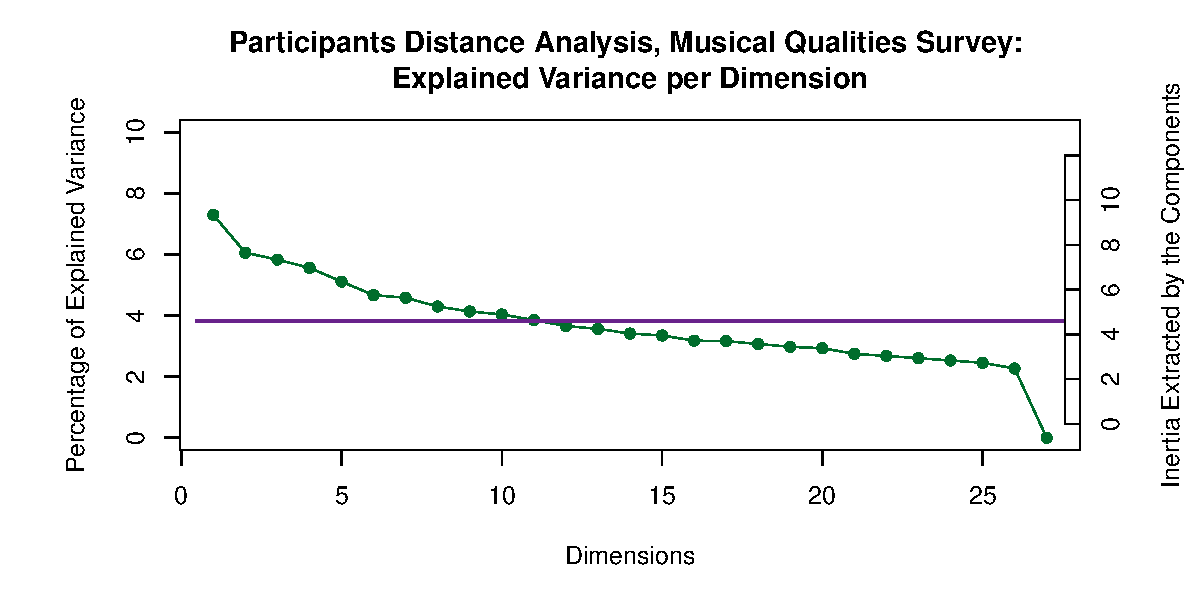
\includegraphics{Music-Descriptor-Space_files/figure-latex/screeRV-1} 

}

\caption{ }\label{fig:screeRV}
\end{figure}

\hypertarget{excerpts}{%
\subsubsection{Excerpts}\label{excerpts}}

The scree plot for the analysis of the musical quality ratings survey (see \ref{fig:scree4excerptsq}) shows the high dimensionality of this space, with the first three dimensions extracting a total of 18.44\%, 14.09\% and 8.81\% respectively, totalling only 41.34\% of the variance. It isn't until we get to the 11th dimension that we see \textgreater80\% of the variance explained. However, given that the assumption in an analysis like this is that the sample is random, it's important to take these numbers with a grain of salt. Music of the type that was presented in this study is by definition not random; in a single excerpt, repetition is common, and some musical qualities are inextricably linked, for example some stylistic elements with genre. As such, we've opted to focus on the first two dimensions in the analysis below.

\begin{figure}

{\centering 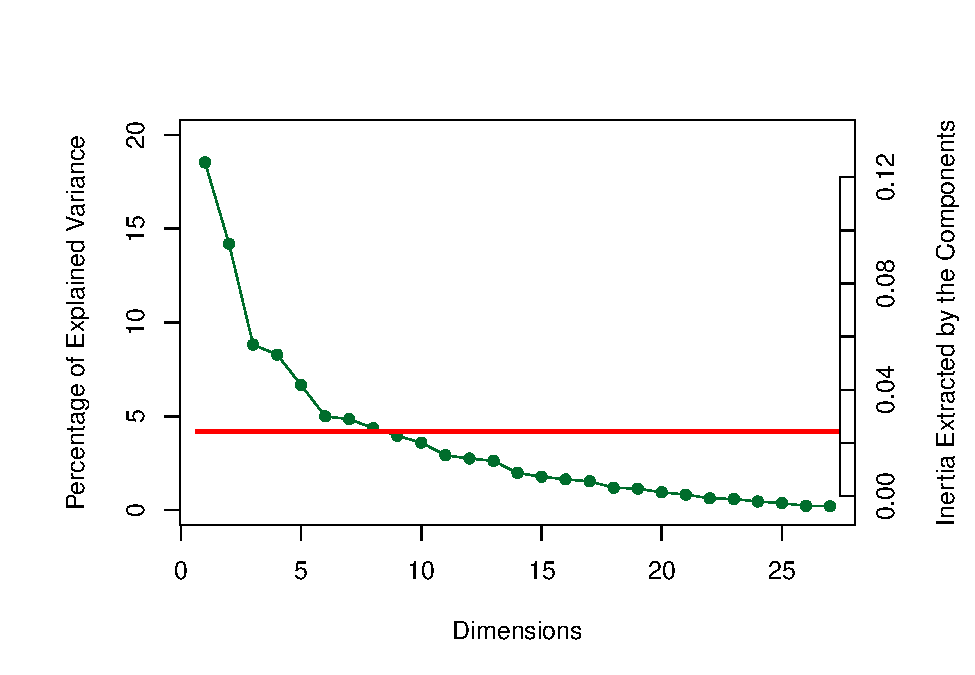
\includegraphics{Music-Descriptor-Space_files/figure-latex/scree4excerptsq-1} 

}

\caption{ }\label{fig:scree4excerptsq}
\end{figure}

Graphing the variable loadings (see \ref{fig:contributionsQ}) on the first two dimensions shows which musical qualities and which musical dimensions contribute the most to the first two dimensions. Because of how CA is calculated, we know that the excerpts that load on the same dimension and direction as the musical qualities are the excerpts that are most associated with those qualities. The contributions shown here are only those that contribute significantly to the first two dimensions, for a table of the complete contributions from the first four dimensions, see supplementary materials.
There are some obvious groups of variables, especially tempo and articulation in the first dimension, with fewer contributions from the dynamics group. The tempo variables, which are a continuum, load from high (tempo.F6 and tempo.F7) in the positive direction to low (tempo.F2 and tempo.F1) in the negative direction. Other contributions are one-off: major harmony, triple meter, classical genre, undulating contour, and disjunct motion. The excerpts that load positively, and are therefore associated with the qualities that load in the positive direction, are all from group 2: Excerpts 4, 13, 23, and 26. The ones that load in the negative direction are from mostly from group 4: Excerpts 7, 10, 24, and 27, with one from group 3, Excerpt 3.

The second dimension seems to dominated by a few groups: harmony, meter, genre, dynamics. The one-offs are slow tempo, ascending contour, and ``no melody.'' The excerpts that load significantly on this dimension are from all four groups. In the positive direction, it's Excerpts 7, 12, 15, and 27 from Group 4, and Excerpt 19 from Group 1. In the negative direction it's Excerpts 2, 3, 11, and 17. All are from group 3 except for Excerpt 2, which is from Group 2. For a full enumeration of contributions, loadings, and boostrap ratios, see table {[}insert table number, also, make up table.{]} in the supplementary materials.

\begin{figure}

{\centering 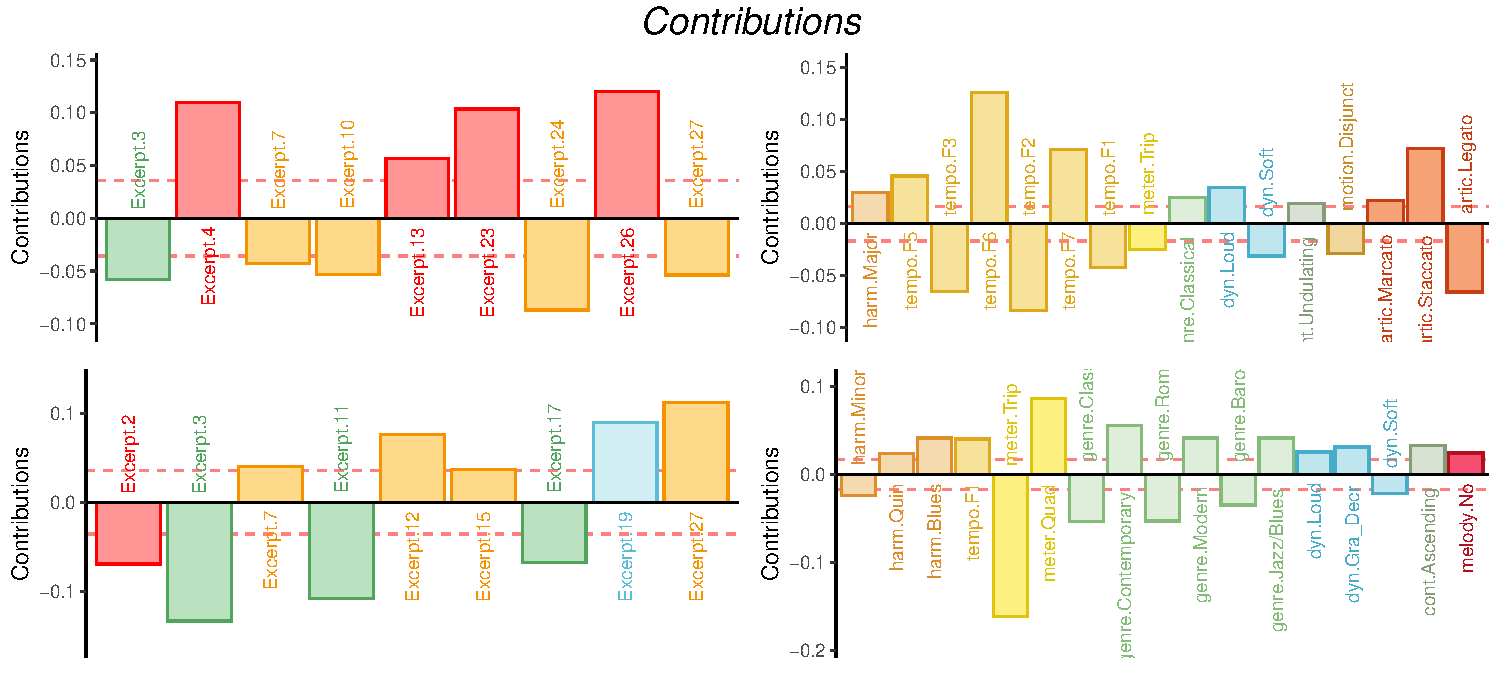
\includegraphics{Music-Descriptor-Space_files/figure-latex/contributionsQ-1} 

}

\caption{ }\label{fig:contributionsQ}
\end{figure}

\hypertarget{discussion}{%
\subsubsection{Discussion}\label{discussion}}

The graph depicted in \ref{fig:factormapswsimplexQ} is a biplot depicting how excerpts and variables plot in the same space. This biplot is possible because of the nature of correspondence analysis. Because the rows and columns of the contingency table X by definition have the same variance, the eigenvalues extracted from X are the same as X\^{}T. Thus the axes on which the factor scores are plotted are the same for both the rows and the columns. However, interpretation requires some discernment. The distance between the excerpts can be interpreted directly as similarity, and the distance between the musical qualities can be interpreted directly as similarity, but the distance between a quality and an excerpt cannot. Instead, the angle between an excerpt and a quality is indicative of their correlation. An angle of 0 indicates a correlation of 1, an angle of 90 indicates a correlation of 0, and an angle of 180 indicates a correlation of -1.
Overall, this helps us to evaluate what contribute to the excerpt groupings. These first two dimensions suggest that the hierarchical cluster analysis \emph{{[}see supplementary materials{]}} revealed groupings roughly according to genre. However, there are two notable outliers. Excerpts 6 and 14 are unique in that they are each the only representative of their respective genres. Excerpt 6 is minimalist, a la Steve Reich, and Excerpt 14 is jazzy. Preliminary versions of this analysis showed that they dominated the 2nd and 3rd dimensions, respectively (see supplementary materials for visualizations). In the plot below, they are included instead as supplementary projections, essentially `out of sample' elements. Their placement on the plot below alludes to the fact that the dimensionality of this space may in fact be related to musical genre or family. Although they dominated the space when included in the sample, they are much closer to the barycenter of the plot when included as out of sample. Were they to fall exactly on the origin, that would suggest that they shared no information whatsoever with the other excerpts included in the analysis. The disparity between their placement on the graph below suggests that they share some information, but there is still a large amount of information that is not accounted for in the factor space below.\\
One perceptual element that is revealed here is that tempo and dynamics seem to contribute, intensity-wise, similarly to the first dimension. The excerpts were not intentionally composed with those characteristics being similar in mind, but it's entirely possible that participants associated high or low arousal levels of the various excerpts and that turned up in the results. For example, given two excerpts of similar tempo, one may have been rated slightly faster if it was also louder, and the other slightly slower if it was quieter. Likewise, given excerpts of similar volume, a faster one may have been rated louder than a slower one. Perception of tempo is also affected by note rate, which is also tied to arousal. In two pieces played at the same tempo, the one with more notes per unit time is more likely to be judged faster than one with fewer.
There are also a few musical elements revealed from the associations. The term staccato means short or light and separated, and the term legato means smooth and connected. The participants in this experiment didn't have access to scores, so they would be judging the excerpts aurally only. With faster excerpts, the notes by definition take up less time, and may be more likely to be judged as light and separate, regardless of what the actual articulation was. Slow tempo and legato are associated in different ways. In terms of performance practice or pedagogy, slow notes are often intended to be connected as smoothly as possible, in order to create a sense of continuity. In terms of genre and harmony, while jazz/blues (on the third dimension) is the most extreme example of this, many genres have harmonies associated with them. For example, the classical genre has fairly structured rules for both harmony and voice leading, but the romantic era relaxed those rules and introduced more complex harmonies. The gradual devolution of those rules and the increase in complexity of harmony continued through the modern and contemporary styles. Although these specific contributions aren't as strong as some of the others, a glance back at the factor scores plot shows that the older genres: baroque, classical, and romantic, are both negative on the 2nd dimension, as are the simpler harmonies of major and minor. Likewise the newer genres: impressionist, modern, and contemporary, load positively on the 2nd dimension, along with the more complex harmonies of chromatic, whole tone, and ambiguous. Historically speaking, the whole tone scale gained great popularity with composers in the impressionist era.
However, because of the nature of this survey, this tells us more about the excerpts specifically than the behavior of the participants. Because the excerpts were composed with the intent of varying across all of these musical dimensions, what we see is a sort of validation that there is, in fact, that variety among these excerpts, and that they are different enough to create a large and varied factor space. It also reveals intrinsic biases in the composer's writing. Two excerpts, 6 and 14, showed an outsized influence on the factor space during preliminary analyses. We determined that this was because they were the only minimalist and jazz excerpts, respectively. They were therefore removed from the analyses and projected as supplementary points. That way we are able to see how they compare to the other excerpts in this factor space without distorting it and dominating one or the other dimensions.

\begin{figure}

{\centering 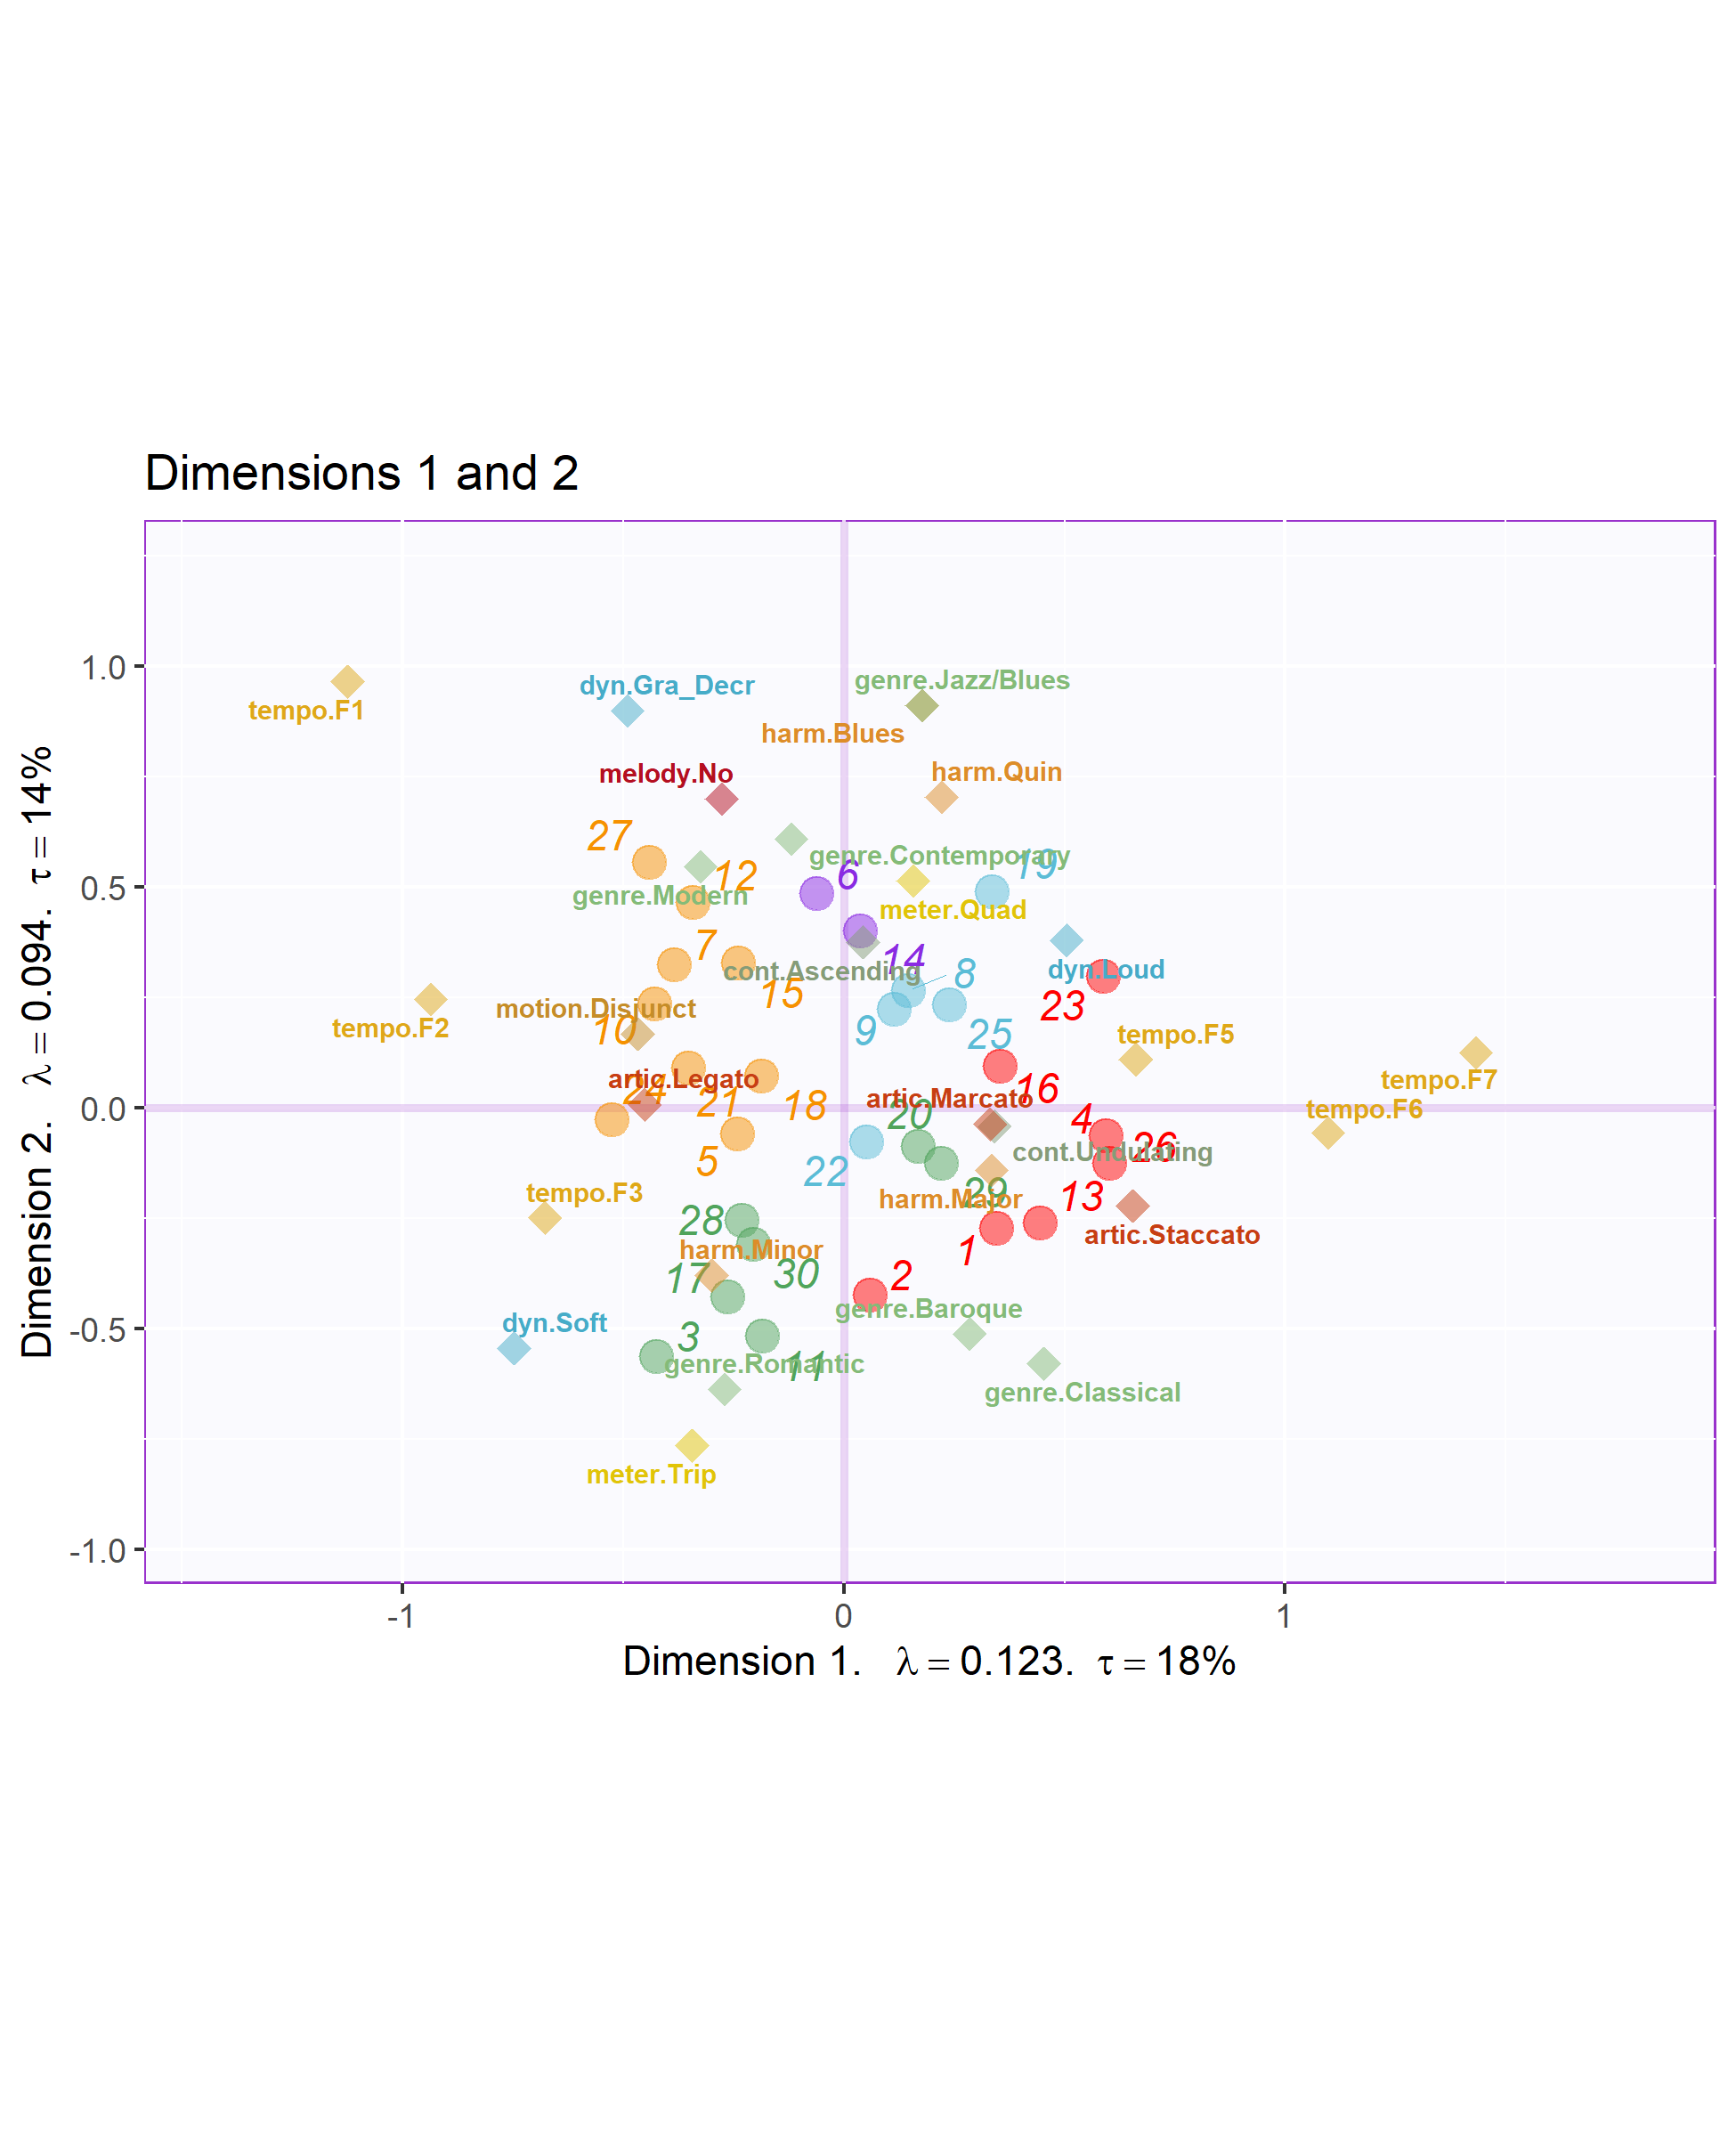
\includegraphics[width=1\linewidth]{Music-Descriptor-Space_files/figure-latex/factormapswsimplexQ-1} 

}

\caption{ }\label{fig:factormapswsimplexQ}
\end{figure}

\hypertarget{experiment-2-musical-adjectives-survey}{%
\subsection{Experiment 2: Musical Adjectives Survey}\label{experiment-2-musical-adjectives-survey}}

\hypertarget{participants-2}{%
\subsubsection{Participants}\label{participants-2}}

The scree plot below shows the explained variance per dimension for the distance analysis of participants in the adjectives survey. Again, having a high number of participants means that the dimensionality is high, and each dimension is only extracting a little bit of variance. However, the first five dimensions all have \(\lambda\) \textgreater{} 1: 1.66, 1.27, 1.13, 1.09, and 1.06, respectively. However, because of the high dimensionality here, the first dimension extracts approximately 3\% of the overall variance, the second dimension extracts approximately 2\%, and each successive dimension extracts incrementally less.

\begin{figure}

{\centering 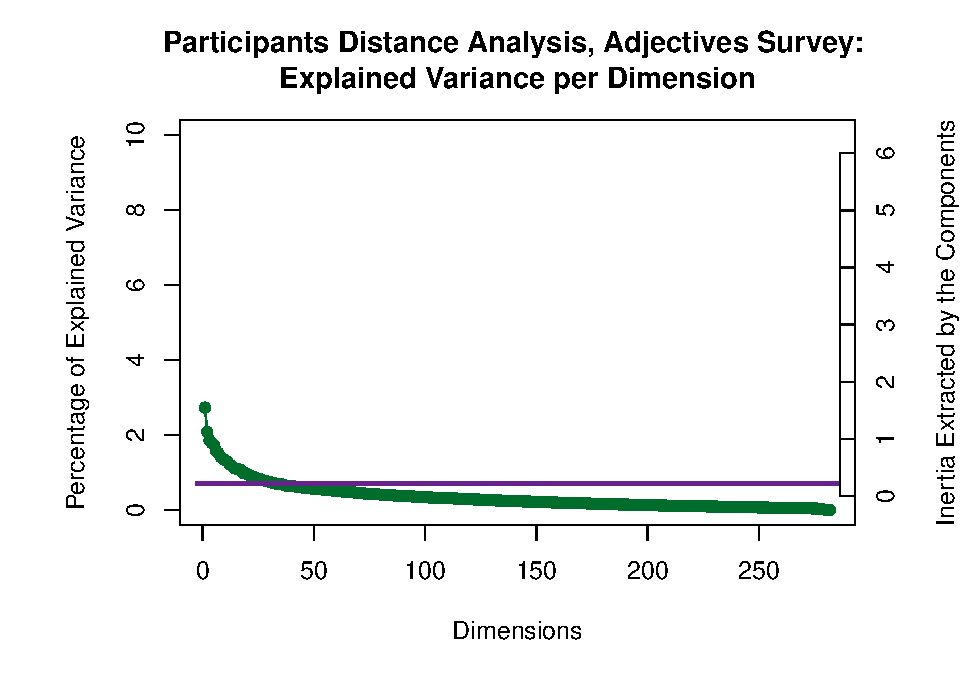
\includegraphics{Music-Descriptor-Space_files/figure-latex/unnamed-chunk-1-1} 

}

\caption{ }\label{fig:unnamed-chunk-1}
\end{figure}

Additionally, this analysis revealed a significant group differences between French and American participants in how they described the excerpts, \(\textit p\). \textless{} .01. This analysis was performed using a distance matrix calculated from the pages of the brick. We calculated a double-centered cross product symmetric distance matrix from the pages of the brick and calculated the factor scores for each participant by calculating the dot product of the eigenvectors and the singular values of that symmetric distance matrix. The factor scores of the participants are plotted below, with with group means and bootstrapped confidence intervals shown for those means. The bootstrapping resampling was performed with 1000 iterations.

\begin{figure}

{\centering 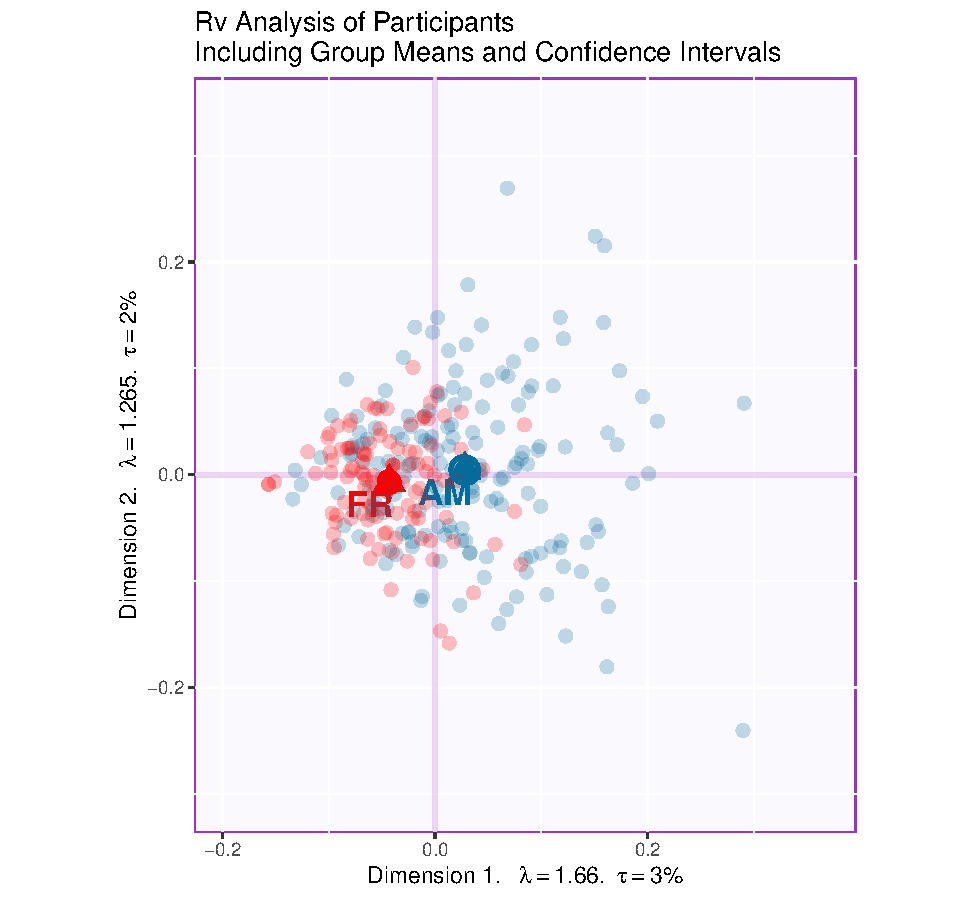
\includegraphics{Music-Descriptor-Space_files/figure-latex/map4RV.A-1} 

}

\caption{ }(\#fig:map4RV.A)
\end{figure}

\hypertarget{excerpts-1}{%
\subsubsection{Excerpts}\label{excerpts-1}}

The plot below shows the explained variance per dimension in the analysis of the excerpts contingency table. Although there are no components with \(\lambda\) \textgreater{} 1, there are two strong dimensions that extract a majority of the variance. The first two dimensions extract 72.25\% of the variance, with the first dimension extracting a majority: 50.05\%, and the second dimension extracting almost a quarter of the overall variance: 50.05\%. This plot also suggests that there are multiple `elbows,' at the 3rd, 5th, and 7th dimensions, respectively, with the third and fourth dimensions forming an `eigen-plane,' of two dimensions which extract similar amounts of variance and should be considered together. For this analysis, however, we're focused on the two first dimensions.
Although excerpts 6 and 14 are outliers in the musical qualities survey, for reasons detailed above, they were not outliers in this analysis. We therefore included them in all of the analyses for Experiment 2.

\begin{figure}

{\centering 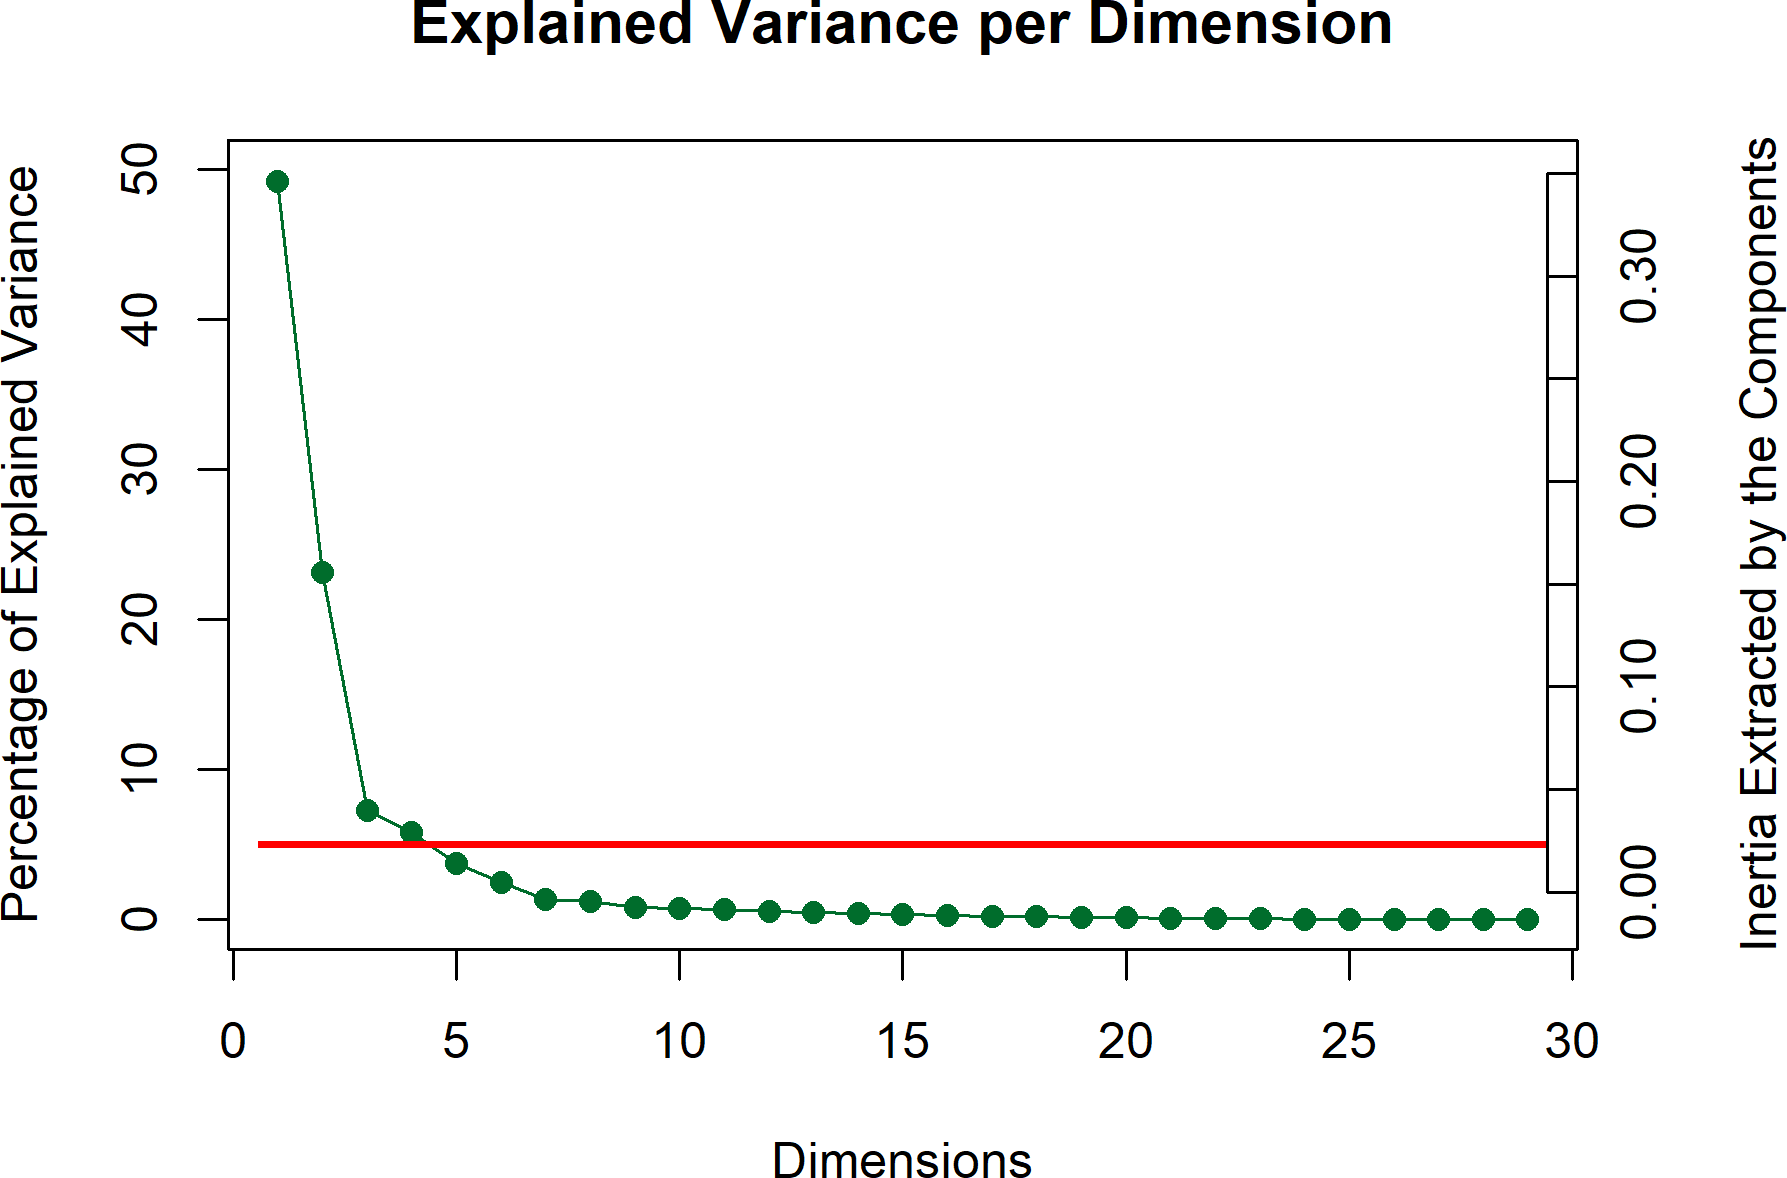
\includegraphics{Music-Descriptor-Space_files/figure-latex/scree4descriptors-1} 

}

\caption{ }\label{fig:scree4descriptors}
\end{figure}

Contributing significantly to the positive end of the first dimension are excerpts from group three (green) and to the negative end are excerpts from group one (yellow). Strong contributions on the positive end of the dimension from the adjectives ``Sad,'' ``Dark,'' ``Melancholy,'' ``Slow,'' ``Mysterious,'' ``Solemn,'' and ``Disturbing.'' The negative end of the first dimension is defined by the adjectives ``Fast,'' ``Happy,'' ``Dancing,'' ``Colorful,'' and ``Bright.''
The second dimension is dominated by excerpts from group 4 (red) in the positive direction and group 2 (blue) in the negative direction. Two excerpts from group 3 also contribute significantly, excerpts 7 in the positive direction and excerpt 10 in the negative direction. The columns contributing strongly in the positive direction are ``Aggressive,'' ``Fast,'' ``Disturbing,'' ``Mysterious,'' ``Surprising'' and ``Complex.'' The columns contributing in the negative direction are ``Warm,''Soft``,''Happy``,''Slow``,''Round``, and''Light". A table showing the full enumeration of all contributions

\begin{figure}

{\centering 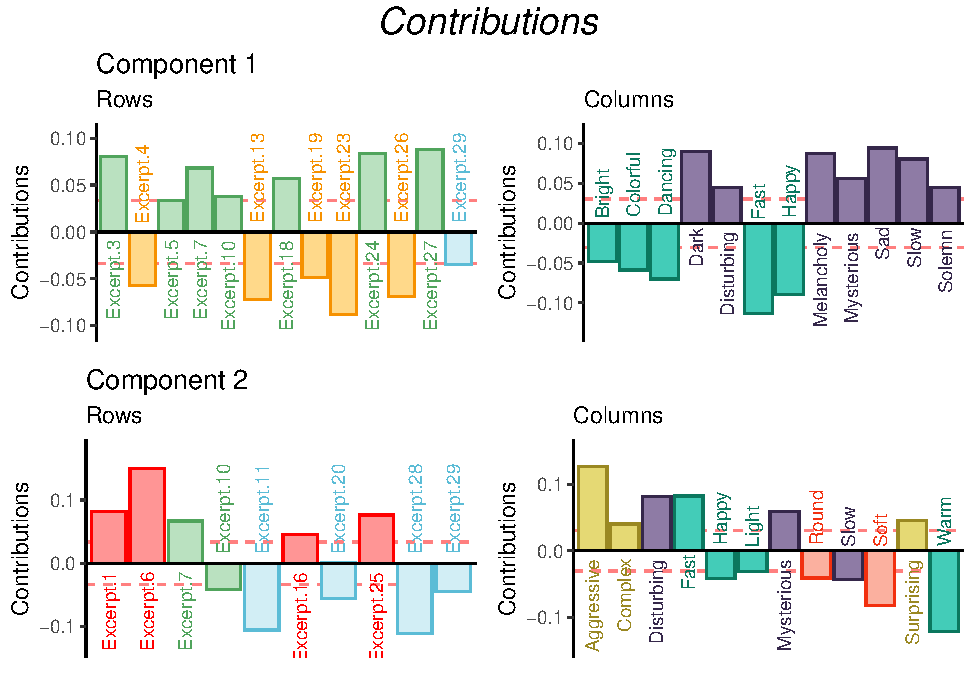
\includegraphics{Music-Descriptor-Space_files/figure-latex/contributions.A-1} 

}

\caption{ }(\#fig:contributions.A)
\end{figure}

\hypertarget{discussion-1}{%
\subsubsection{Discussion}\label{discussion-1}}

The factor maps below show the row and column factor scores for the american and french participants. These are once again symmetric plots, interpretation is the same as the factor plot for the musical qualities. There's a clear valence-arousal plane apparent for both, and in both cases valence seems to define the first dimension and arousal defines the second dimension. However, the difference in the amount of variance extracted by the first two dimensions between the french and american participants is notable. The french data show a weaker first dimension but a stronger second dimension relative to the americans, both in terms of variance extracted (tau), effect size (lambda).

There are also differences in how the adjectives and the excerpts are distributed in the space. One clear example is that Excerpt 6 is in quadrant four in the american plot, but quadrant one in the french. This is a small change, but it suggests that the french participants were more likely to assign negative valence to this excerpt, and American Participants were more likely to assign positive valence. For the adjectives, `bright' and `dancing' are directly on top of one another in the American plot, but there is some space between the two in the French plot. It's possible that this reflects the idea that although the meaning is shared between languages, there are semantic or associational differences between the words.

\begin{verbatim}
## [1] "Preprocessed the Rows of the data matrix using:  None"
## [1] "Preprocessed the Columns of the data matrix using:  Center_1Norm"
## [1] "Preprocessed the Tables of the data matrix using:  MFA_Normalization"
## [1] "Preprocessing Completed"
## [1] "Optimizing using:  None"
## [1] "Processing Complete"
\end{verbatim}

\begin{verbatim}
## [1] "Preprocessed the Rows of the data matrix using:  None"
## [1] "Preprocessed the Columns of the data matrix using:  Center_1Norm"
## [1] "Preprocessed the Tables of the data matrix using:  MFA_Normalization"
## [1] "Preprocessing Completed"
## [1] "Optimizing using:  None"
## [1] "Processing Complete"
\end{verbatim}

Additionally, a post-hoc Multiple Factor Analysis revealed the following in terms of the semantic and perceptual differences between French and American participants.

\begin{figure}

{\centering 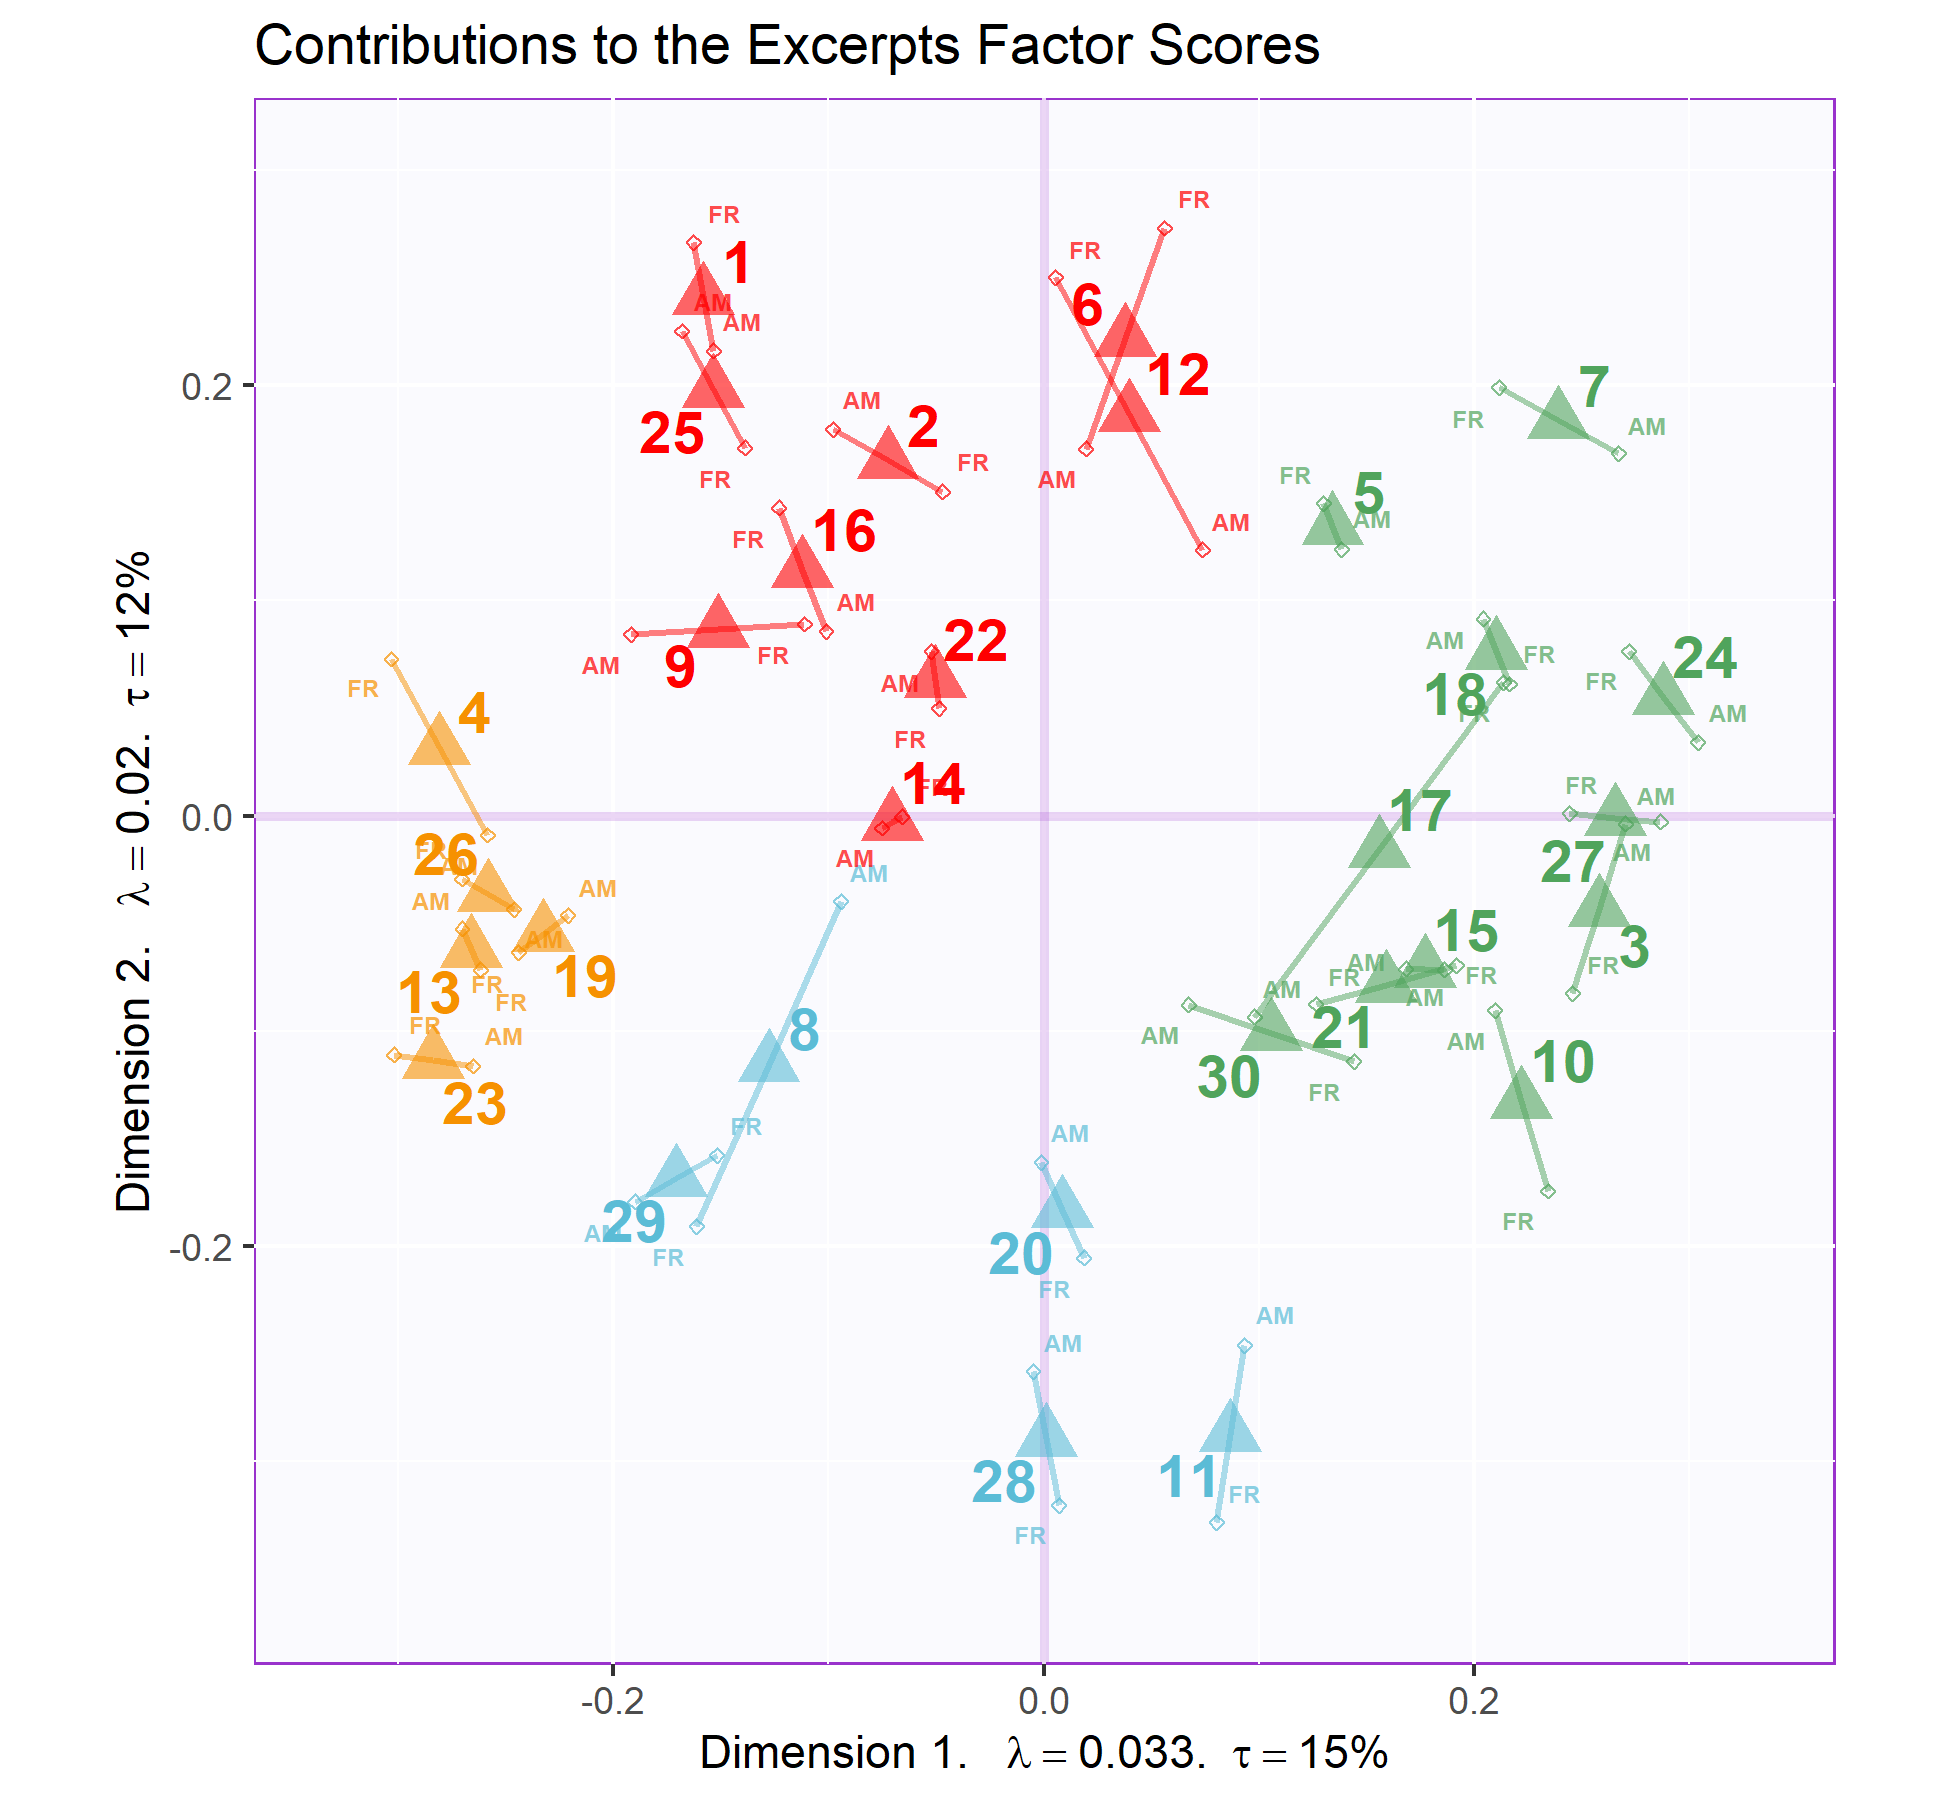
\includegraphics{Music-Descriptor-Space_files/figure-latex/mfasbs-1} 

}

\caption{ }\label{fig:mfasbs-1}
\end{figure}
\begin{figure}

{\centering 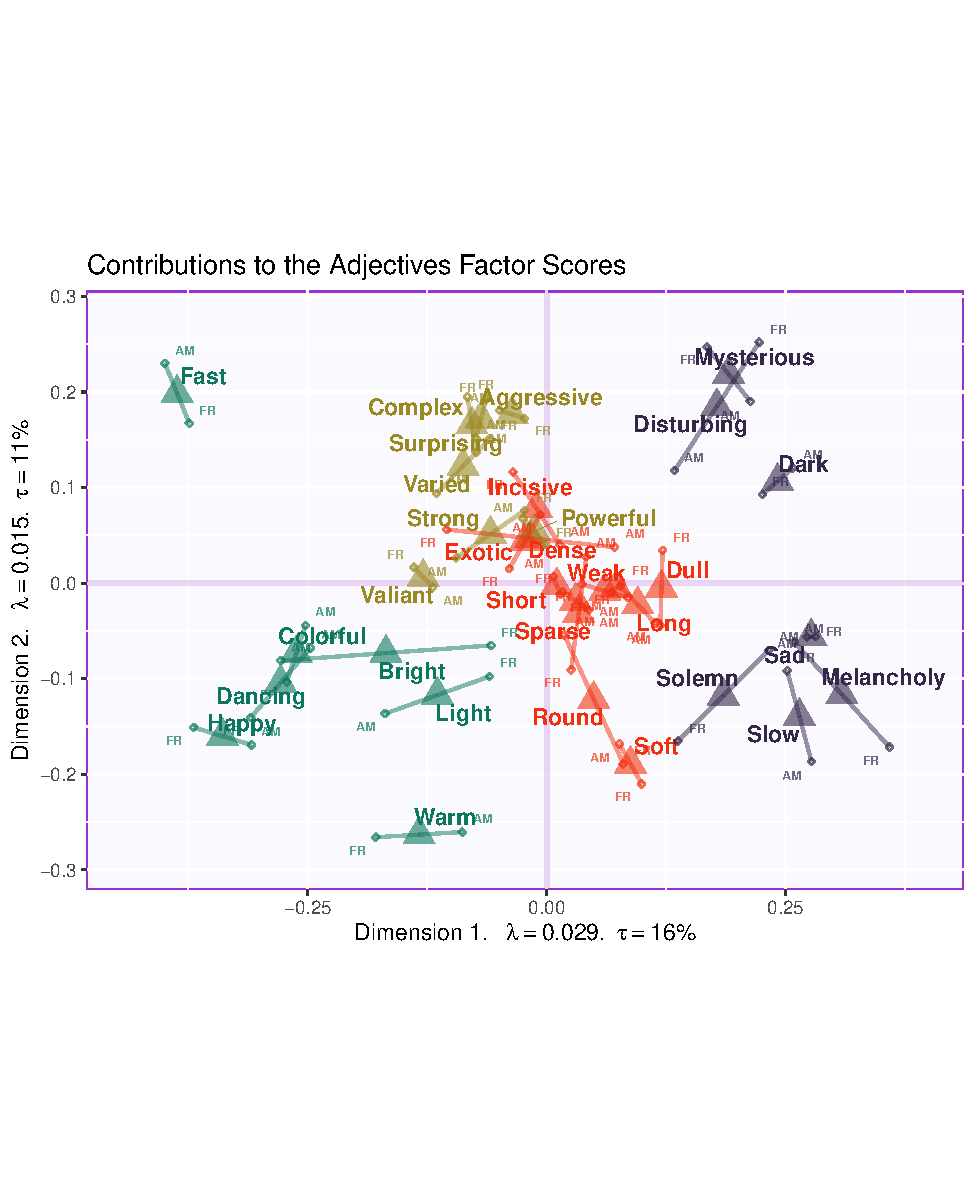
\includegraphics{Music-Descriptor-Space_files/figure-latex/mfasbs-2} 

}

\caption{ }\label{fig:mfasbs-2}
\end{figure}
\begin{figure}

{\centering 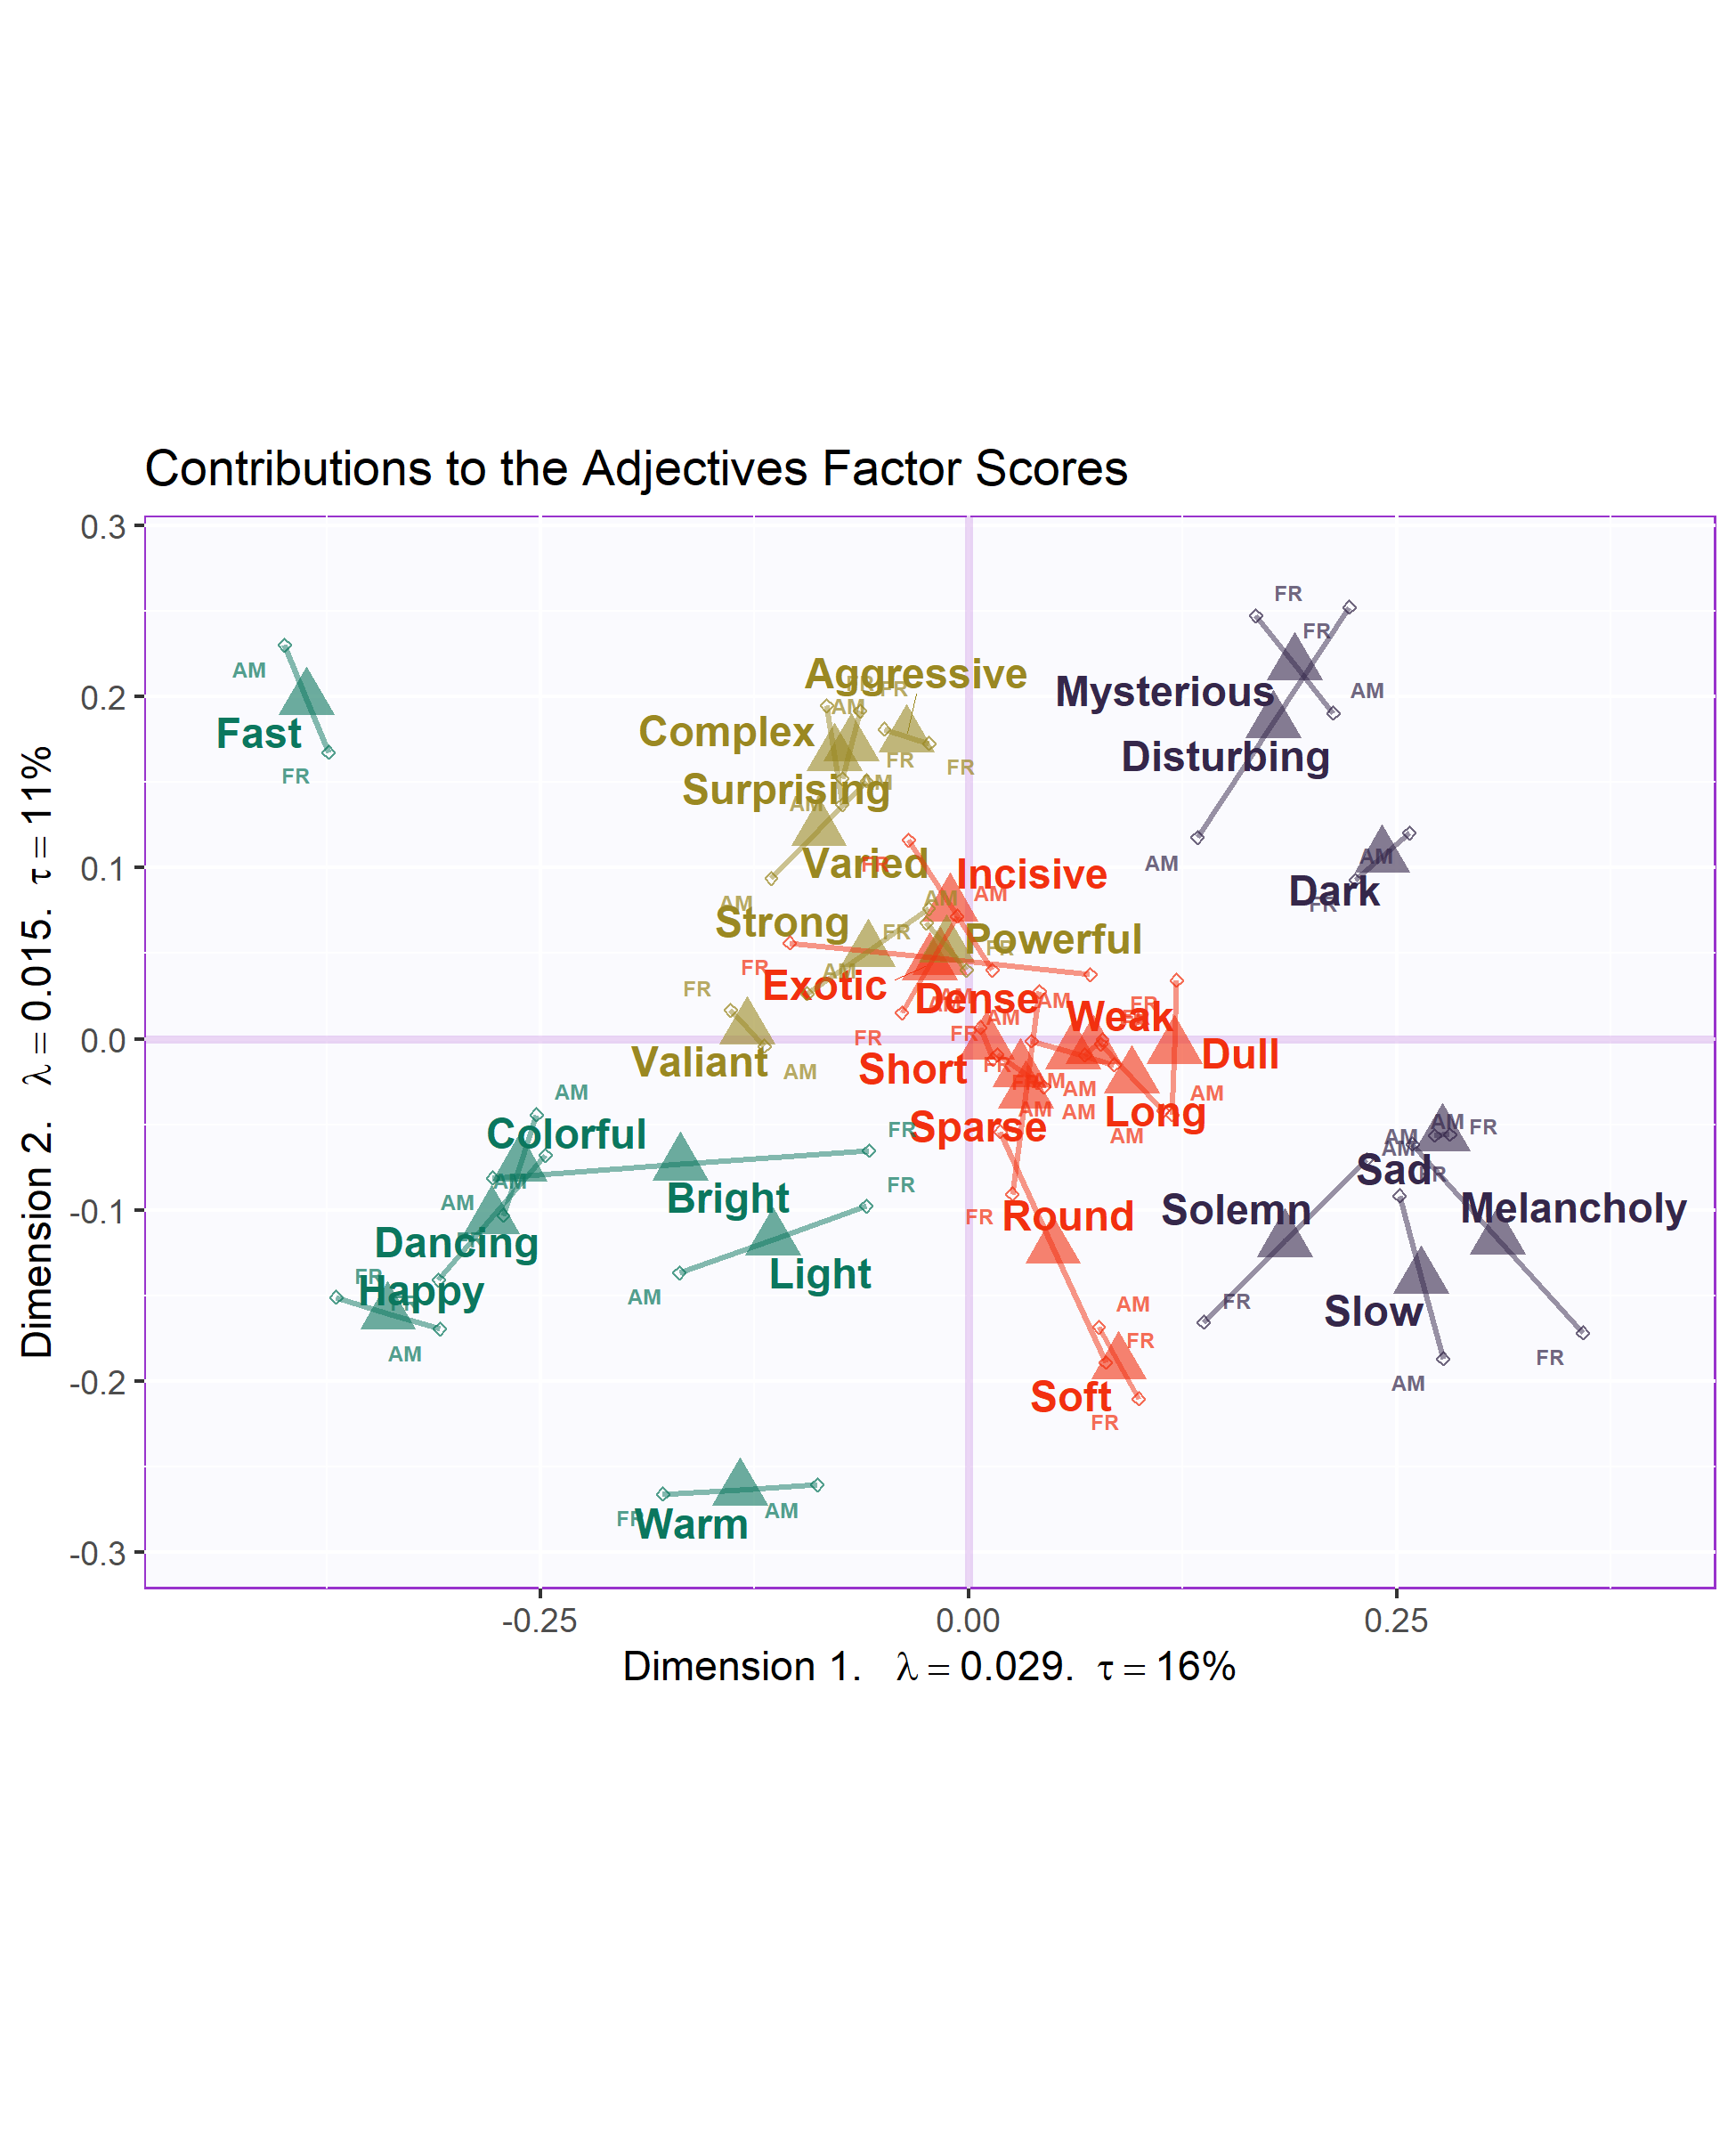
\includegraphics{Music-Descriptor-Space_files/figure-latex/mfasbs-3} 

}

\caption{ }\label{fig:mfasbs-3}
\end{figure}

\hypertarget{experiment-3-combined-surveys}{%
\subsection{Experiment 3: Combined Surveys}\label{experiment-3-combined-surveys}}

The final analysis was performed using a PLSC, which extracts covariance between two tables in the form of \emph{latent variables}. See (\textbf{Krishnan2011?}) for a review. This technique is commonly used in brain imaging to identify which brain regions are activated during a behavioral task ((\textbf{Krishnan2011?})). In our context, the PLSC extracts the information that is shared between the adjectives ratings and the musical dimensions ratings. The visualizations below allow us to see which variables from each of the two tables correspond with one another, or which adjectives are associated with which musical dimensions. Even though both individual tables have their own factor spaces above, plotting the common factor space between the two should allow us to see which excerpts are separated from one another using data from both surveys. Additionally, the contributions and loadings will show us which variables are responsible for creating or defining that space.

The latent variables represent the strongest similarities between the two tables. This experiment requires that one of the dimensions of the two data tables being used are the same. For two matrices, X and Y, where X is an i x j matrix and Y is an i x k matrix, we transpose X such that the two are conformable, and take the dot product. We then have a j x k matrix for which each cell represents the

This analysis revealed two dimensions that extracted the majority of the variance (83.60\%). Of that total extracted by the first two dimensions, the first dimension extracted 64.35\% and the second dimension extracted 19.26\%. The scree plot below shows that it's possible that there are two elbows in this graph, at the 3rd and 5th dimensions. The 3rd and 4th dimensions are also significant, extracting 6.02\% and 3.67\% of the variance, respectively. Interpretations of the third dimension and beyond is beyond the scope of this paper, but seeing that there are multiple significant dimensions beyond the second does provide a possible future direction using this method.

\begin{figure}

{\centering 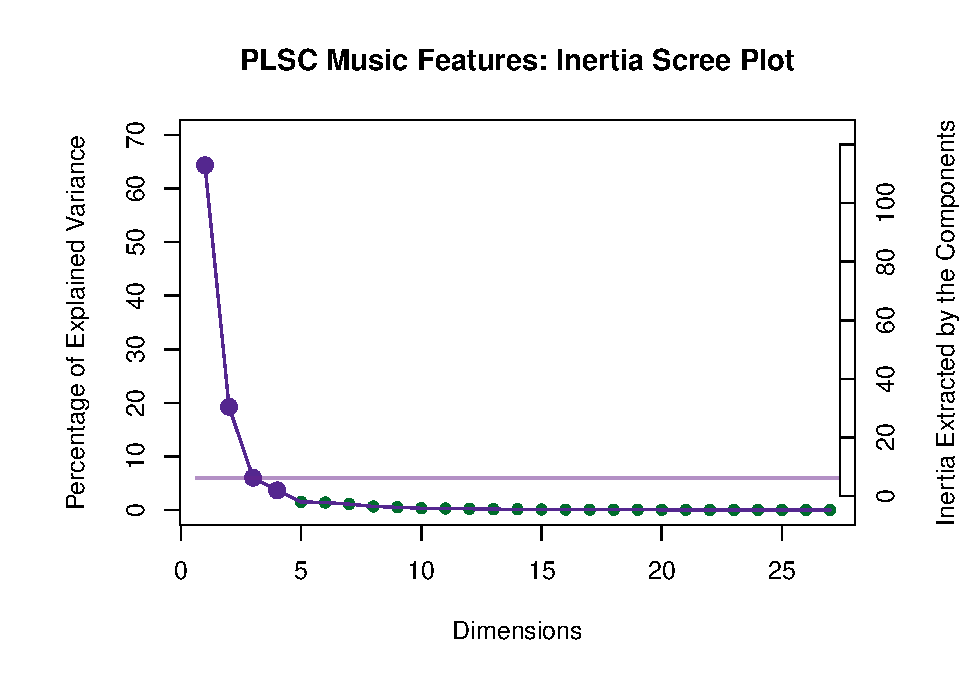
\includegraphics{Music-Descriptor-Space_files/figure-latex/screePLSC-1} 

}

\caption{ }\label{fig:screePLSC}
\end{figure}

The plot below shows which variables from each data table load the most on the first and second dimensions. For the purposes of this visualization, we are showing only the variables for which 70\% or more of the variance is explained. The nature of the PLSC also suggests that these are the variables that are most associated with one another between the two tables. The strongest signal on the first dimension juxtaposes the slow and legato musical qualities in the positive direction with the fast, staccato, marcato, and conjunct musical qualities in the negative direction. The adjectives associated with the qualities in the positive direction are ``Dark,'' ``Dull,'' ``Long,'' ``Melancholy,'' ``Sad,'' ``Slow,'' ``Solemn,'' and ``Weak.'' The adjectives associated with the negative direction are ``Bright,'' ``Colorful,'' ``Dancing,'' ``Fast,'' ``Happy,'' and ``Light.''\\
The second dimension identified in the positive direction major harmony and mezzo dynamics, associated with ``Light,'' ``Round,'' ``Soft,'' and ``Warm.'' The negative direction is driven by the impressionist genre being associated with ``Aggressive,'' ``Complex,'' ``Dense,'' ``Disturbing,'' ``Powerful,'' and ``Surprising.''

\begin{figure}

{\centering 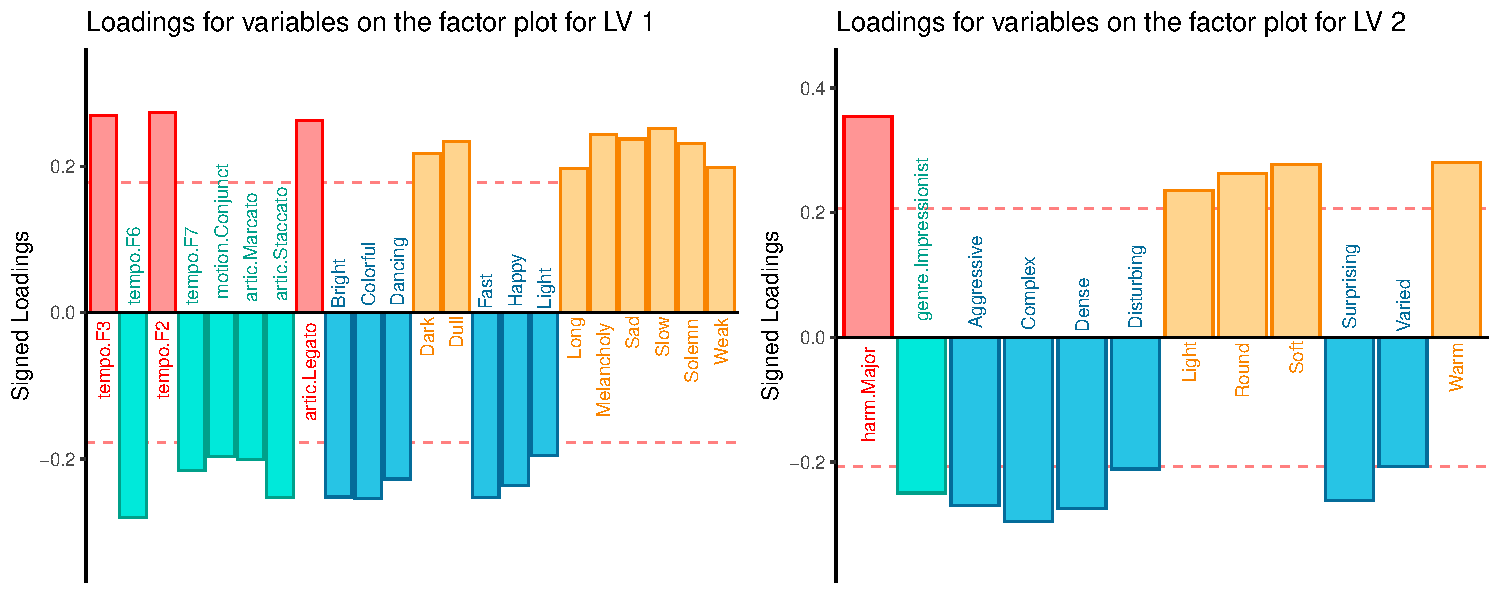
\includegraphics{Music-Descriptor-Space_files/figure-latex/loadingsplsc-1} 

}

\caption{ }\label{fig:loadingsplsc}
\end{figure}

Contributions and loadings are similar, but not exactly the same. Here were see that there are quite a few more variables that contribute significantly to these dimensions than for which a significant portion of the variance is explained. We do see similar groups, however: on the first dimension, the tempo variables are contributing significantly, along with some from harmony, density, genre, dynamics, motion, range, and articulation. The adjectives contributing significantly are Bright, colorful, Dancing, Fast, Happy, Light, and Valiant in the negative direction, and Dark, Dull, Long, Melancholy, Monotonous, Sad, Slow, Solemn, and Weak in the positive direction. What's notable here is that while some of these adjectives did contribute significantly in the plots above, some didn't contribute much at all and fell near the barycenter of the factor plot. We also see that this juxtaposes some negatively and positively valenced adjectives, which allows us to identify which of the musical qualities contributes to the valence dimension.
The second dimension tells us a similar story. Here we see more of the harmony variables, along with one tempo variable, some density, genre, a few dynamics, contour, motion, range, and articulation. The adjectives contributing negatively are Aggressive, Complex, Dense, Disturbing, Incisive, Mysterious, Powerful, Surprising, and Varied, and those contributing positively are Light, Round, Soft, Transparent, and Warm. Again we see similar effects of variables that may not have contributed significantly to their respective plots above, but are contributing significantly here. Also, this second latent variable seems to be defining the arousal dimension.

\begin{figure}

{\centering 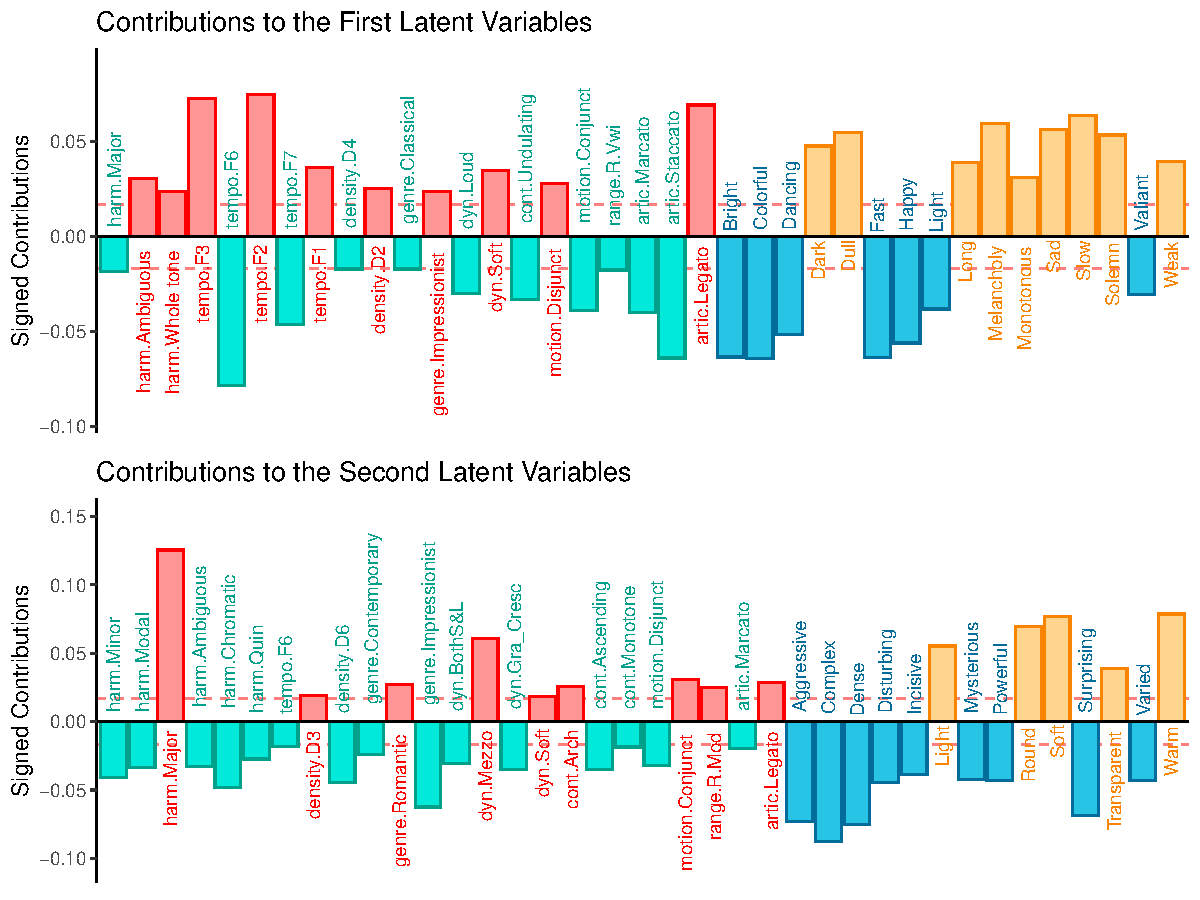
\includegraphics{Music-Descriptor-Space_files/figure-latex/contsplsc-1} 

}

\caption{ }\label{fig:contsplsc}
\end{figure}

\hypertarget{discussion-2}{%
\subsubsection{Discussion}\label{discussion-2}}

The factor score plots for these show that the first two latent variables extracted by the analysis effectively separate the groups of excerpts. This factor plot shows us how the strongest correlated signal between the two data tables separates Excerpts groups 2 and 3, but groups 1 and two didn't contribute much to this dimension, instead contributing to the 2nd latent variables. The second latent variable separates Groups 1 and 4, with Groups 2 and 3 more barycentric. This suggests that, generally speaking, the excerpts that were clustered in groups 2 and 3 are those that could be defined by positive and negative valence, respectively, and those in groups 1 and 4 would be defined more by high and low arousal. That being said, these excerpts are not defined \emph{exclusively} along these dimensions, but rather more by one than the other. For example, excerpt 26 is characterized by being one the most extreme examples of positive valence, but doesn't score as highly on the arousal dimension, similarly with excerpt 27 with negative valence. This is contrasted with excerpt 7, which is one of the most negatively valenced stimuli, but also scores very high on arousal, although the barycenter for that group is near the origin of that plot.

\begin{figure}

{\centering 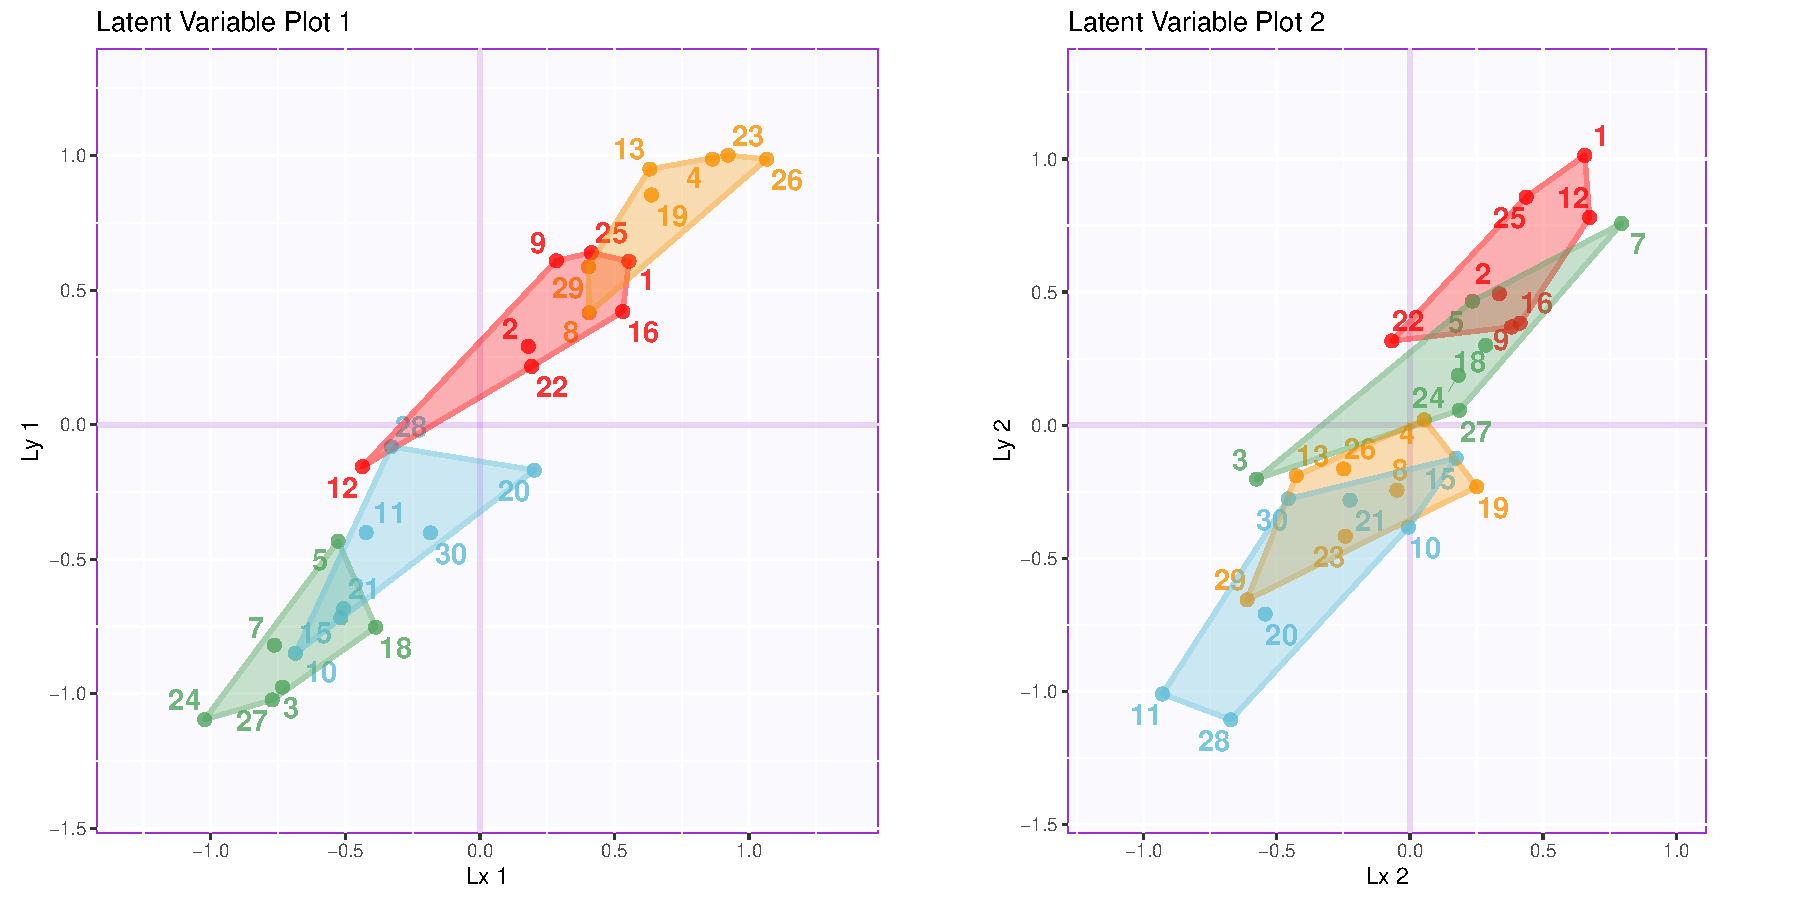
\includegraphics{Music-Descriptor-Space_files/figure-latex/factorplotsPLSC-1} 

}

\caption{ }\label{fig:factorplotsPLSC}
\end{figure}

\hypertarget{general-discussion}{%
\section{General Discussion}\label{general-discussion}}

Although this study was designed to evaluate the sensory or cognitive response to music, and not specifically the emotional response, there is significant overlap in the results observed here and the results of the work investigating musical and emotion. The appearance of the valence arousal plane in the results of experiment 2 was not unexpected, even though the adjectives we selected were not intended to be explicitly emotional. This goes to show difficult it is to avoid any emotional content when selecting descriptors, and from another perspective, how much emotional contagion the music examples carry. Overall, this supports the idea that the first two dimensions on which music is judged holistically are valence and arousal.
Some of the results discussed in Experiment 1 require more explanation. In experiment 1, there was an issue of having two individual excerpts dominate the factor space, which did not happen in experiment 2. Because of the nature of CA, the musical qualities survey is not robust to outliers. One of the ways in which CA is different from PCA is that PCA is usually unweighted. Because CA includes the masses of the columns and the weights of the rows in the calculations, information that is common gravitates towards the barycenter of the factor space, while rare information (the stuff that's actually interesting) tends to pop out. Unfortunately that means that if there is an item or element in the data that is unique or otherwise very different from every other item in the dataset, we end up with a situation like the one in Experiment 1, where excerpts 6 and 14 dominate the factor space. Using supplementary projections, as illustrated above, is a good way to extract the information that those outliers share with the other elements in the dataset without having them dominate the visualization of the factor space. The reason that this happened for experiment 1 and not experiment 2 is that the adjectives don't measure explicit musical dimensions. While the musical qualities surveys captured a result that may have characterized by 4-6 factors, each approximating genre and the qualities associated with that genre, the adjectives/descriptors survey had no such restriction. The general affective space captures an entirely different set of information about the music from the musical qualitative space.\\
The hierarchical cluster analyses revealed different groupings in how the stimuli were rated between the two surveys. The PLSC then showed that when including both sets of data, there was a coherent interpretable factor space on which the excerpts were plotted. There are a number of ways to further disambiguate the results of the surveys. One way would be to run a MFA, similar to the one above that plotted the difference between French and American raters on the adjective survey. This would allow for a number of different interpretations. Firstly, it would calculate the overall factor space for the excerpts, including all of the data from both surveys, without separating out the first and second dimensions to plot them separately. It would also identify the specific partial factor scores for each of the data tables within that factor space that would allow for the interpretation of the relative differences between the data tables. The drawback to both of these, however, is that unlike the separate correspondence analyses we ran above, where the row and column scores can be plotted in the same space, neither MFA nor the PLSC allow for that type of visualization.

\hypertarget{limitations-future-directions}{%
\subsection{Limitations \& future directions}\label{limitations-future-directions}}

Although we evaluate the scores and ratings of participants from different countries, we recognize that the issue of multiculturality is not addressed to a significant degree in this study. The sample was still largely students, and France and the United States share similar musical cultures. To truly address this question, it would be very interesting to include participants from multiple, contrasting musical cultures, with languages that are more distinct than English and French. This presents new problems, however, as the specific musical qualities included in the surveys may not all apply to or translate well to other musical cultures. Harmony, for example, is a concept that is developed to a significant degree in western music, but melody or rhythm may be the fundamental focus of other musical cultures (cite patel here? I forget.).
Another question that fell beyond the scope of this study is the concept of semantic drift between languages. Although illustrated in \ref{fig:mfasbs}, the source of the differences between French and American participants falls beyond the scope of this paper. We humbly hazard to guess that some of the sources of the difference include aspects of perception that extend beyond the musical. These could be linguistic sources, such as the physical characteristics of the words themselves, the cultural associations with the words, or the frequency of use in either language. Diving more into those questions of linguistics and semantic drift between languages would be a fascinating future study.
Another interesting study would be to repeat this study using adjectives from specific domains or that that avoid explicit emotional or musical content, to see how music maps onto different sensory spaces. For example, `moist,' `slimy,' `dry,' `puckered,' `smooth.' Although some of these adjectives may carry musical weight, in the context of other words that all relate to haptic sensation, it may provide some interesting feedback regarding how the music maps into other sensory domains.
Finally, using these studies may provide pilot work for the way in which people without language react to music, nonverbal autistic people, for example. Whereas this study explicitly uses language as an interlocutor for music perception, it offers insight into ways to better communicate with people who do not have that ability.

\hypertarget{conclusions}{%
\section{Conclusions}\label{conclusions}}

By developing investigative paradigms that are accessible on mobile platforms, and that reduce participant demand while maintaining rigor and integrity, we are likely to be able to reach a much greater subset of the population. If we are able to pair this kind of data gathering with appropriate exploratory analysis, we can target much more effectively where we might investigate with more traditional hypothesis testing. The analyses literature to date in this domain has focused on a fairly small subset of the multivariate analyses available to investigate these questions. As presented here, the number of ways that exist to analyze the data from a single set of experiments is considerable, and the results of each analysis illuminate different areas of the question or problem at hand. It would behoove us as researchers to seek out and use as many of these analyses as possible to open up new avenues of investigation and to possibly expand the analyses of the data we've already collected.

\newpage

\hypertarget{references}{%
\section{References}\label{references}}

\begingroup
\setlength{\parindent}{-0.5in}
\setlength{\leftskip}{0.5in}

\hypertarget{refs}{}
\begin{CSLReferences}{0}{0}
\end{CSLReferences}

\endgroup


\end{document}
